%%
% Copyright (c) 2017 - 2020, Pascal Wagler;
% Copyright (c) 2014 - 2020, John MacFarlane
%
% All rights reserved.
%
% Redistribution and use in source and binary forms, with or without
% modification, are permitted provided that the following conditions
% are met:
%
% - Redistributions of source code must retain the above copyright
% notice, this list of conditions and the following disclaimer.
%
% - Redistributions in binary form must reproduce the above copyright
% notice, this list of conditions and the following disclaimer in the
% documentation and/or other materials provided with the distribution.
%
% - Neither the name of John MacFarlane nor the names of other
% contributors may be used to endorse or promote products derived
% from this software without specific prior written permission.
%
% THIS SOFTWARE IS PROVIDED BY THE COPYRIGHT HOLDERS AND CONTRIBUTORS
% "AS IS" AND ANY EXPRESS OR IMPLIED WARRANTIES, INCLUDING, BUT NOT
% LIMITED TO, THE IMPLIED WARRANTIES OF MERCHANTABILITY AND FITNESS
% FOR A PARTICULAR PURPOSE ARE DISCLAIMED. IN NO EVENT SHALL THE
% COPYRIGHT OWNER OR CONTRIBUTORS BE LIABLE FOR ANY DIRECT, INDIRECT,
% INCIDENTAL, SPECIAL, EXEMPLARY, OR CONSEQUENTIAL DAMAGES (INCLUDING,
% BUT NOT LIMITED TO, PROCUREMENT OF SUBSTITUTE GOODS OR SERVICES;
% LOSS OF USE, DATA, OR PROFITS; OR BUSINESS INTERRUPTION) HOWEVER
% CAUSED AND ON ANY THEORY OF LIABILITY, WHETHER IN CONTRACT, STRICT
% LIABILITY, OR TORT (INCLUDING NEGLIGENCE OR OTHERWISE) ARISING IN
% ANY WAY OUT OF THE USE OF THIS SOFTWARE, EVEN IF ADVISED OF THE
% POSSIBILITY OF SUCH DAMAGE.
%%

%%
% This is the Eisvogel pandoc LaTeX template.
%
% For usage information and examples visit the official GitHub page:
% https://github.com/Wandmalfarbe/pandoc-latex-template
%%

% Options for packages loaded elsewhere
\PassOptionsToPackage{unicode}{hyperref}
\PassOptionsToPackage{hyphens}{url}
\PassOptionsToPackage{dvipsnames,svgnames*,x11names*,table}{xcolor}
%
\documentclass[
  ngerman,
  paper=a4,
,captions=tableheading
]{scrartcl}
\usepackage{lmodern}
\usepackage{setspace}
\setstretch{1.2}
\usepackage{amssymb,amsmath}
\usepackage{ifxetex,ifluatex}
\ifnum 0\ifxetex 1\fi\ifluatex 1\fi=0 % if pdftex
  \usepackage[T1]{fontenc}
  \usepackage[utf8]{inputenc}
  \usepackage{textcomp} % provide euro and other symbols
\else % if luatex or xetex
  \usepackage{unicode-math}
  \defaultfontfeatures{Scale=MatchLowercase}
  \defaultfontfeatures[\rmfamily]{Ligatures=TeX,Scale=1}
\fi
% Use upquote if available, for straight quotes in verbatim environments
\IfFileExists{upquote.sty}{\usepackage{upquote}}{}
\IfFileExists{microtype.sty}{% use microtype if available
  \usepackage[]{microtype}
  \UseMicrotypeSet[protrusion]{basicmath} % disable protrusion for tt fonts
}{}
\makeatletter
\@ifundefined{KOMAClassName}{% if non-KOMA class
  \IfFileExists{parskip.sty}{%
    \usepackage{parskip}
  }{% else
    \setlength{\parindent}{0pt}
    \setlength{\parskip}{6pt plus 2pt minus 1pt}}
}{% if KOMA class
  \KOMAoptions{parskip=half}}
\makeatother
\usepackage{xcolor}
\definecolor{default-linkcolor}{HTML}{A50000}
\definecolor{default-filecolor}{HTML}{A50000}
\definecolor{default-citecolor}{HTML}{4077C0}
\definecolor{default-urlcolor}{HTML}{4077C0}
\IfFileExists{xurl.sty}{\usepackage{xurl}}{} % add URL line breaks if available
\IfFileExists{bookmark.sty}{\usepackage{bookmark}}{\usepackage{hyperref}}
\hypersetup{
  pdftitle={unlernOS für Dich Leitfaden},
  pdfauthor={Joe Doe},
  pdflang={de-de},
  hidelinks,
  breaklinks=true,
  pdfcreator={LaTeX via pandoc with the Eisvogel template}}
\urlstyle{same} % disable monospaced font for URLs
\usepackage[margin=2.5cm,includehead=true,includefoot=true,centering,]{geometry}
\usepackage[export]{adjustbox}
\usepackage{graphicx}
\usepackage{longtable,booktabs}
% Correct order of tables after \paragraph or \subparagraph
\usepackage{etoolbox}
\makeatletter
\patchcmd\longtable{\par}{\if@noskipsec\mbox{}\fi\par}{}{}
\makeatother
% Allow footnotes in longtable head/foot
\IfFileExists{footnotehyper.sty}{\usepackage{footnotehyper}}{\usepackage{footnote}}
\makesavenoteenv{longtable}
% add backlinks to footnote references, cf. https://tex.stackexchange.com/questions/302266/make-footnote-clickable-both-ways
\usepackage{footnotebackref}
\usepackage{graphicx}
\makeatletter
\def\maxwidth{\ifdim\Gin@nat@width>\linewidth\linewidth\else\Gin@nat@width\fi}
\def\maxheight{\ifdim\Gin@nat@height>\textheight\textheight\else\Gin@nat@height\fi}
\makeatother
% Scale images if necessary, so that they will not overflow the page
% margins by default, and it is still possible to overwrite the defaults
% using explicit options in \includegraphics[width, height, ...]{}
\setkeys{Gin}{width=\maxwidth,height=\maxheight,keepaspectratio}
% Make links footnotes instead of hotlinks:
\DeclareRobustCommand{\href}[2]{#2\footnote{\url{#1}}}
\setlength{\emergencystretch}{3em}  % prevent overfull lines
\providecommand{\tightlist}{%
  \setlength{\itemsep}{0pt}\setlength{\parskip}{0pt}}
\setcounter{secnumdepth}{3}

% Make use of float-package and set default placement for figures to H.
% The option H means 'PUT IT HERE' (as  opposed to the standard h option which means 'You may put it here if you like').
\usepackage{float}
\floatplacement{figure}{H}

\ifxetex
    % See issue https://github.com/reutenauer/polyglossia/issues/127
  \renewcommand*\familydefault{\sfdefault}
    % Load polyglossia as late as possible: uses bidi with RTL langages (e.g. Hebrew, Arabic)
  \usepackage{polyglossia}
  \setmainlanguage[]{german}
\else
  \usepackage[shorthands=off,main=ngerman]{babel}
\fi

\title{unlernOS für Dich Leitfaden}
\usepackage{etoolbox}
\makeatletter
\providecommand{\subtitle}[1]{% add subtitle to \maketitle
  \apptocmd{\@title}{\par {\large #1 \par}}{}{}
}
\makeatother
\subtitle{Die Kunst des lebenslangen, selbstgesteuerten Lernens}
\author{Joe Doe}
\date{Version 1.6 (31.03.2020)}



%%
%% added
%%

%
% language specification
%
% If no language is specified, use English as the default main document language.
%



%
% for the background color of the title page
%
\usepackage{pagecolor}
\usepackage{afterpage}
\usepackage[margin=2.5cm,includehead=true,includefoot=true,centering]{geometry}

%
% break urls
%
\PassOptionsToPackage{hyphens}{url}

%
% When using babel or polyglossia with biblatex, loading csquotes is recommended
% to ensure that quoted texts are typeset according to the rules of your main language.
%
\usepackage{csquotes}

%
% captions
%
\definecolor{caption-color}{HTML}{777777}
\usepackage[font={stretch=1.2}, textfont={color=caption-color}, position=top, skip=4mm, labelfont=bf, singlelinecheck=false, justification=raggedright]{caption}
\setcapindent{0em}

%
% blockquote
%
\definecolor{blockquote-border}{RGB}{221,221,221}
\definecolor{blockquote-text}{RGB}{119,119,119}
\usepackage{mdframed}
\newmdenv[rightline=false,bottomline=false,topline=false,linewidth=3pt,linecolor=blockquote-border,skipabove=\parskip]{customblockquote}
\renewenvironment{quote}{\begin{customblockquote}\list{}{\rightmargin=0em\leftmargin=0em}%
\item\relax\color{blockquote-text}\ignorespaces}{\unskip\unskip\endlist\end{customblockquote}}

%
% Source Sans Pro as the de­fault font fam­ily
% Source Code Pro for monospace text
%
% 'default' option sets the default
% font family to Source Sans Pro, not \sfdefault.
%
\ifnum 0\ifxetex 1\fi\ifluatex 1\fi=0 % if pdftex
    \usepackage[default]{sourcesanspro}
  \usepackage{sourcecodepro}
  \else % if not pdftex
    \usepackage[default]{sourcesanspro}
  \usepackage{sourcecodepro}

  % XeLaTeX specific adjustments for straight quotes: https://tex.stackexchange.com/a/354887
  % This issue is already fixed (see https://github.com/silkeh/latex-sourcecodepro/pull/5) but the
  % fix is still unreleased.
  % TODO: Remove this workaround when the new version of sourcecodepro is released on CTAN.
  \ifxetex
    \makeatletter
    \defaultfontfeatures[\ttfamily]
      { Numbers   = \sourcecodepro@figurestyle,
        Scale     = \SourceCodePro@scale,
        Extension = .otf }
    \setmonofont
      [ UprightFont    = *-\sourcecodepro@regstyle,
        ItalicFont     = *-\sourcecodepro@regstyle It,
        BoldFont       = *-\sourcecodepro@boldstyle,
        BoldItalicFont = *-\sourcecodepro@boldstyle It ]
      {SourceCodePro}
    \makeatother
  \fi
  \fi

%
% heading color
%
\definecolor{heading-color}{RGB}{40,40,40}
\addtokomafont{section}{\color{heading-color}}
% When using the classes report, scrreprt, book,
% scrbook or memoir, uncomment the following line.
%\addtokomafont{chapter}{\color{heading-color}}

%
% variables for title, author and date
%
\usepackage{titling}
\title{unlernOS für Dich Leitfaden}
\author{Joe Doe}
\date{Version 1.6 (31.03.2020)}

%
% tables
%

\definecolor{table-row-color}{HTML}{F5F5F5}
\definecolor{table-rule-color}{HTML}{999999}

%\arrayrulecolor{black!40}
\arrayrulecolor{table-rule-color}     % color of \toprule, \midrule, \bottomrule
\setlength\heavyrulewidth{0.3ex}      % thickness of \toprule, \bottomrule
\renewcommand{\arraystretch}{1.3}     % spacing (padding)


%
% remove paragraph indention
%
\setlength{\parindent}{0pt}
\setlength{\parskip}{6pt plus 2pt minus 1pt}
\setlength{\emergencystretch}{3em}  % prevent overfull lines

%
%
% Listings
%
%


%
% header and footer
%
\usepackage{fancyhdr}

\fancypagestyle{eisvogel-header-footer}{
  \fancyhead{}
  \fancyfoot{}
  \lhead[Version 1.6 (31.03.2020)]{unlernOS für Dich Leitfaden}
  \chead[]{}
  \rhead[unlernOS für Dich Leitfaden]{Version 1.6 (31.03.2020)}
  \lfoot[\thepage]{Joe Doe}
  \cfoot[]{}
  \rfoot[Joe Doe]{\thepage}
  \renewcommand{\headrulewidth}{0.4pt}
  \renewcommand{\footrulewidth}{0.4pt}
}
\pagestyle{eisvogel-header-footer}

%%
%% end added
%%

\begin{document}

%%
%% begin titlepage
%%
\begin{titlepage}
\newgeometry{left=6cm}
\definecolor{titlepage-color}{HTML}{00ff00}
\newpagecolor{titlepage-color}\afterpage{\restorepagecolor}
\newcommand{\colorRule}[3][black]{\textcolor[HTML]{#1}{\rule{#2}{#3}}}
\begin{flushleft}
\noindent
\\[-1em]
\color[HTML]{ffffff}
\makebox[0pt][l]{\colorRule[ffffff]{1.3\textwidth}{4pt}}
\par
\noindent

{
  \setstretch{1.4}
  \vfill
  \noindent {\huge \textbf{\textsf{unlernOS für Dich Leitfaden}}}
    \vskip 1em
  {\Large \textsf{Die Kunst des lebenslangen, selbstgesteuerten
Lernens}}
    \vskip 2em
  \noindent {\Large \textsf{Joe Doe}}
  \vfill
}

\noindent
\includegraphics[width=300pt, left]{src/images/lernOS-logo-white-4000px.png}

\textsf{Version 1.6 (31.03.2020)}
\end{flushleft}
\end{titlepage}
\restoregeometry

%%
%% end titlepage
%%



{
\setcounter{tocdepth}{3}
\tableofcontents
\newpage
}
\hypertarget{uxfcber-lernos}{%
\section{Über lernOS}\label{uxfcber-lernos}}

lernOS ist eine Methode zur Selbstorganisation für Menschen, die im 21.
Jahrhundert leben und arbeiten. Um heute erfolgreich zu sein, muss man
ständig lernen, sich organisieren und weiterentwickeln. Niemand sonst
ist für diesen Prozess verantwortlich. Man muss sich selber darum
kümmern (selbstgesteuertes, lebenslanges Lernen).

Der Trend Working Out Loud bedeutet, die eigene Arbeit sichtbar zu
machen und über die eigene Arbeit zu erzählen, um Vernetzung zu
ermöglichen und Hilfe aus dem Netzwerk zu erhalten. Als Plattform kommen
oft interne und externe soziale Netzwerke zum Einsatz. Gerade wenn es um
den Transport von Wissen zu komplexen Themen oder Emotionen geht,
reichen kurze Texte oft nicht aus. Hier eignen sich Audio- und
Video-Formate wie Screencasts, Erklärvideos und Podcasts besser.

Podcasts haben hierbei den Vorteil, dass sie viel einfacher zu
produzieren sind, als Videos. Außerdem können Podcasts an Orten
konsumiert werden, an denen die Nutzung von Videos schwierig ist
(Pendler, im Auto, im Flugzeug, beim Spazieren etc.). Mit diesem lernOS
Leitfaden lernt ihr in einem Learning Sprint, selber Podcast zu machen
und zu veröffentlichen. Ihr könnt den Podcasting Lernpfad alleine
durchlaufen oder in einem Learning Circle mit 4-5 anderen Personen.

@simondueckert

\textbf{Lizenz:}

lernOS Leitfäden stehen unter der Lizenz
\href{https://creativecommons.org/licenses/by/4.0/deed.de}{Creative
Commons Namensnennung 4.0 International} (CC BY 4.0):


\includegraphics{./tex2pdf.-af94b87e0fdb9aa6/d18286abe9c5f984f58813bfa721e63381b92a7a.png}

\textbf{Du darfst:}

\begin{itemize}
\tightlist
\item
  \textbf{Teilen} - das Material in jedwedem Format oder Medium
  vervielfältigen und weiterverbreiten.
\item
  \textbf{Bearbeiten} - das Material remixen, verändern und darauf
  aufbauen und zwar für beliebige Zwecke, sogar kommerziell.
\end{itemize}

\textbf{Unter folgenden Bedingungen:}

\begin{itemize}
\tightlist
\item
  \textbf{Namensnennung} - Du musst angemessene Urheber- und
  Rechteangaben machen, einen Link zur Lizenz beifügen und angeben, ob
  Änderungen vorgenommen wurden. Diese Angaben dürfen in jeder
  angemessenen Art und Weise gemacht werden, allerdings nicht so, dass
  der Eindruck entsteht, der Lizenzgeber unterstütze gerade Sie oder
  Ihre Nutzung besonders.
\item
  \textbf{Keine weiteren Einschränkungen} - Du darst keine zusätzlichen
  Klauseln oder technische Verfahren einsetzen, die anderen rechtlich
  irgendetwas untersagen, was die Lizenz erlaubt.
\end{itemize}

\hypertarget{basics}{%
\section{Basics}\label{basics}}

Wir stehen vor enormen Herausforderungen, die durch Globalisierung,
Digitalisierung sowie schnelle technologische und wissenschaftliche
Entwicklung angetrieben werden. Gleichzeitig bieten uns diese
Veränderungen viele neue Entwicklungsmöglichkeiten. Die Zukunft ist
ungewiss und wir können Sie nicht vorhersagen. Wir müssen also offen und
bereit dafür sein und sie gemeinsam gestalten (Quelle:
\href{https://www.oecd.org/education/2030}{Learning Framework 2030}). Um
durch die sogenannte
\href{https://en.wikipedia.org/wiki/Volatility,_uncertainty,_complexity_and_ambiguity}{VUCA}-Welt
des 21. Jahrhunderts voller Volatilität, Unsicherheit, Komplexität und
Mehrdeutigkeit zu navigieren, müssen sich Teenager, Studenten,
Fachleute, Manager und Führungskräfte ständig weiterentwickeln. Jeder
muss Fähigkeiten wie Kreativität, kritisches Denken, Kommunikation und
Kollaboration erlernen. Digital Literacy ist die Kompetenz, mit Hilfe
digitaler Tools lesen und schreiben, sowie an gemeinsamen Aktivitäten
teilhaben zu können. Sie ist wichtig, um digitale Werkzeuge produktiv
einsetzen zu können. Die Motivation für die persönliche Entwicklung
sollte dabei mehr sein, als einen gut bezahlten Job zu bekommen oder
Profit zu machen. Jeder sollte sich um das eigene Wohlergehen, aber auch
das Wohl seiner Freunde und Familie, seiner Communities und der
Gesellschaft kümmern. Wir müssen lernen, welches Wissen, Fähigkeiten,
Denkweisen, Einstellungen, Werte, Methoden und Werkzeuge wir brauchen,
um gemeinsam eine bessere Zukunft zu gestalten.

lernOS kann dir helfen, Dich fit für das 21. Jahrhundert zu machen.
lernOS hilft Dir, deine Aktivitäten zu organisieren und bewusst aus
jeder Aktion zu lernen. Es fördert außerdem die Vernetzung mit anderen
Menschen, damit du nicht jedes Rad neu erfinden und jeden Fehler
wiederholen musst.

Und das Beste ist: lernOS ist frei, offen und leicht zu verstehen.
Starte heute damit!

\hypertarget{noch-mehr-basics}{%
\subsection{Noch mehr Basics}\label{noch-mehr-basics}}

\begin{itemize}
\tightlist
\item
  Erstens
\item
  Zweitens \#\# lernOS Sprints: Lebenslanges Lernen in 13-wöchigen
  Timeboxen
\end{itemize}

lernOS wird in Zeiträumen von 13 Wochen, die wie bei
\href{https://scrumguides.org}{Scrum} Learning Sprints genannt werden,
praktiziert. Normalerweise laufen die Sprints jeweils in einem Quartal
des Jahres. Der Rhythmus kann bei Bedarf angepasst werden. Ein Sprint
kann alleine (lernOS Solist), zu zweit (lernOS Tandem) oder in einer
Gruppe von 4-5 Personen (lernOS Circle) durchlaufen werden.

\begin{figure}
\centering
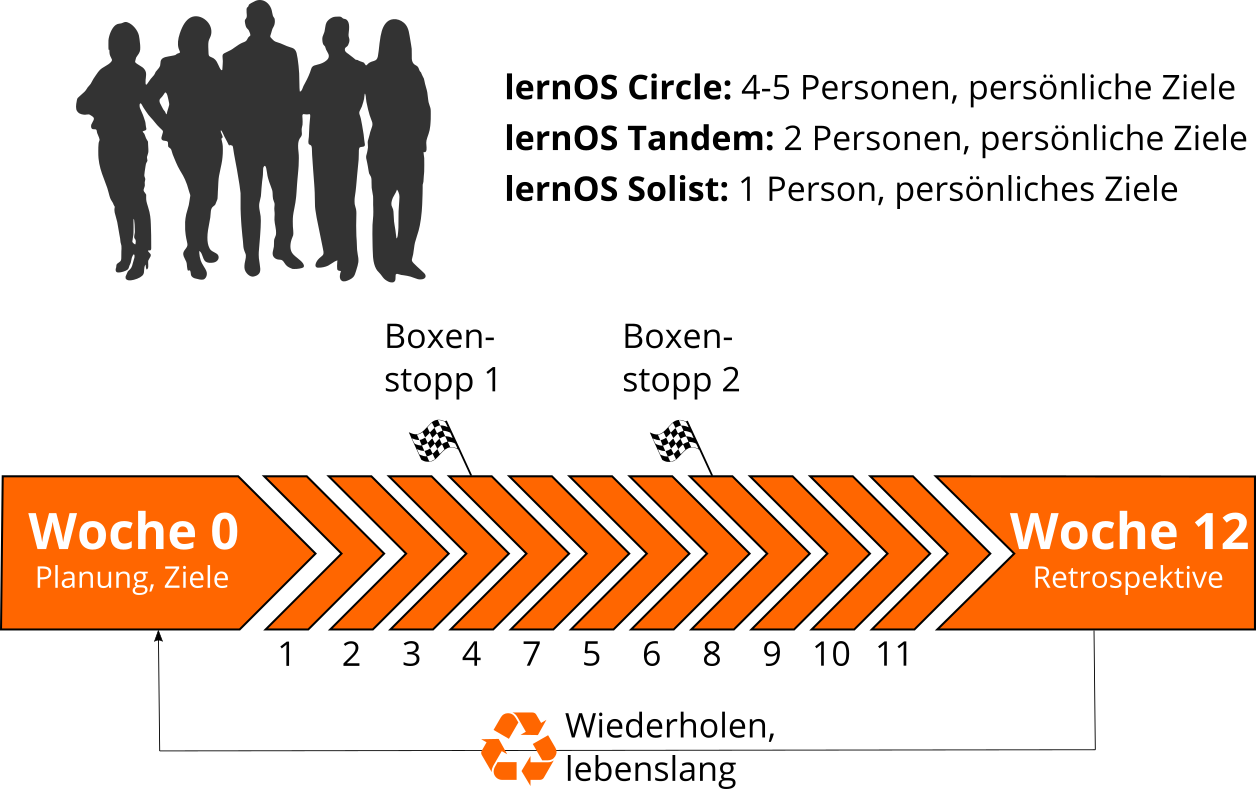
\includegraphics{./tex2pdf.-af94b87e0fdb9aa6/80c28d15a479ebb119ba5c36bcbcf681c76609a4.png}
\caption{lernOS Sprint}
\end{figure}

So läuft ein lernOS Sprint ab:

\begin{itemize}
\tightlist
\item
  \textbf{Woche 0:} Die Sprint Planung. Versteht jeder die
  Vorgehensweise? Wann wird der wöchentliche Termin (Weekly)
  stattfinden? Welcher Lernpfad wird für den Sprint gewählt? Bei lernOS
  Tandems und Circles: Wird das Weekly als persönliches Treffen oder
  virtuell stattfinden? Welche Tools werden für die Kommunikation und
  Dokumentation verwendet? Ist jeder in der Lage, die Tools zu
  verwenden?
\item
  \textbf{Wochen 1-11:} Es wird an den Zielen und gewünschten
  Ergebnissen gearbeitet und der Fortschritt im Weekly kritisch
  reflektiert. Ein Lernpfad schlägt Übungen vor, die wie bei
  \href{https://coderdojo.com}{CoderDojos} Katas genannt werden. Für
  Einsteiger*innen (NOOBs) stehen drei Lernpfade zur Verfügung:
  WOL-Lernpfad (offenes und vernetztes Arbeiten und Lernen),
  OKR-Lernpfad (zielgerichtetes und fokussiertes Arbeiten und Lernen)
  und GTD-Lernpfad (stressfreies und produktives Arbeiten und Lernen).
  Die Empfehlung ist, je Sprint nur ein Lernpfad auszuwählen und in
  Lerntandems oder Circles die Lernpfade nicht zu mischen. Die beiden
  Boxenstopps in Woche 4 und Woche 8 helfen zu sehen, ob noch alle auf
  dem richtigen Weg sind.
\item
  \textbf{Woche 12 mit der Retrospektive:} Review der finalen Ergebnisse
  des Sprints und Retrospektive des gesamten Prozesses. Bei Lerntandems
  und Circles: Die Beteiligten entscheiden, ob sie für einen weiteren
  Sprint zusammen bleiben wollen.
\end{itemize}

In Schule und Hochschule wird der Takt des Lernens durch Schuljahre und
Semester vorgegeben. Um das Lernen danach selbstorganisiert zu
stukturieren, werden die lernOS Sprints im Extremfall bis zum eigenen
Lebensende eingeplant (von der Wiege bis zur Bahre), so wie das
\href{https://www.inc.com/magazine/19970201/1169.html}{auch schon Peter
Drucker} praktiziert hat.

\hypertarget{lernos-wheel-mindset-skillset-und-toolset}{%
\subsection{lernOS Wheel: Mindset, Skillset und
Toolset}\label{lernos-wheel-mindset-skillset-und-toolset}}

Die Beherrschung der VUCA-Welt des 21. Jahrhunderts erfordert Offenheit
für Veränderungen und neue Ansätze. Es gibt eine Menge von Werkzeugen
und Methoden. Aber wenn du nicht offen bist, sie auszuprobieren, zu
experimentieren und zu scheitern, wird der Erfolg ausbleiben. Wie die
Leute mit den ``quadratischen Rädern'' im Bild unten, sind wir oft zu
beschäftigt, um die neuen Chancen zu sehen.

\begin{figure}
\centering
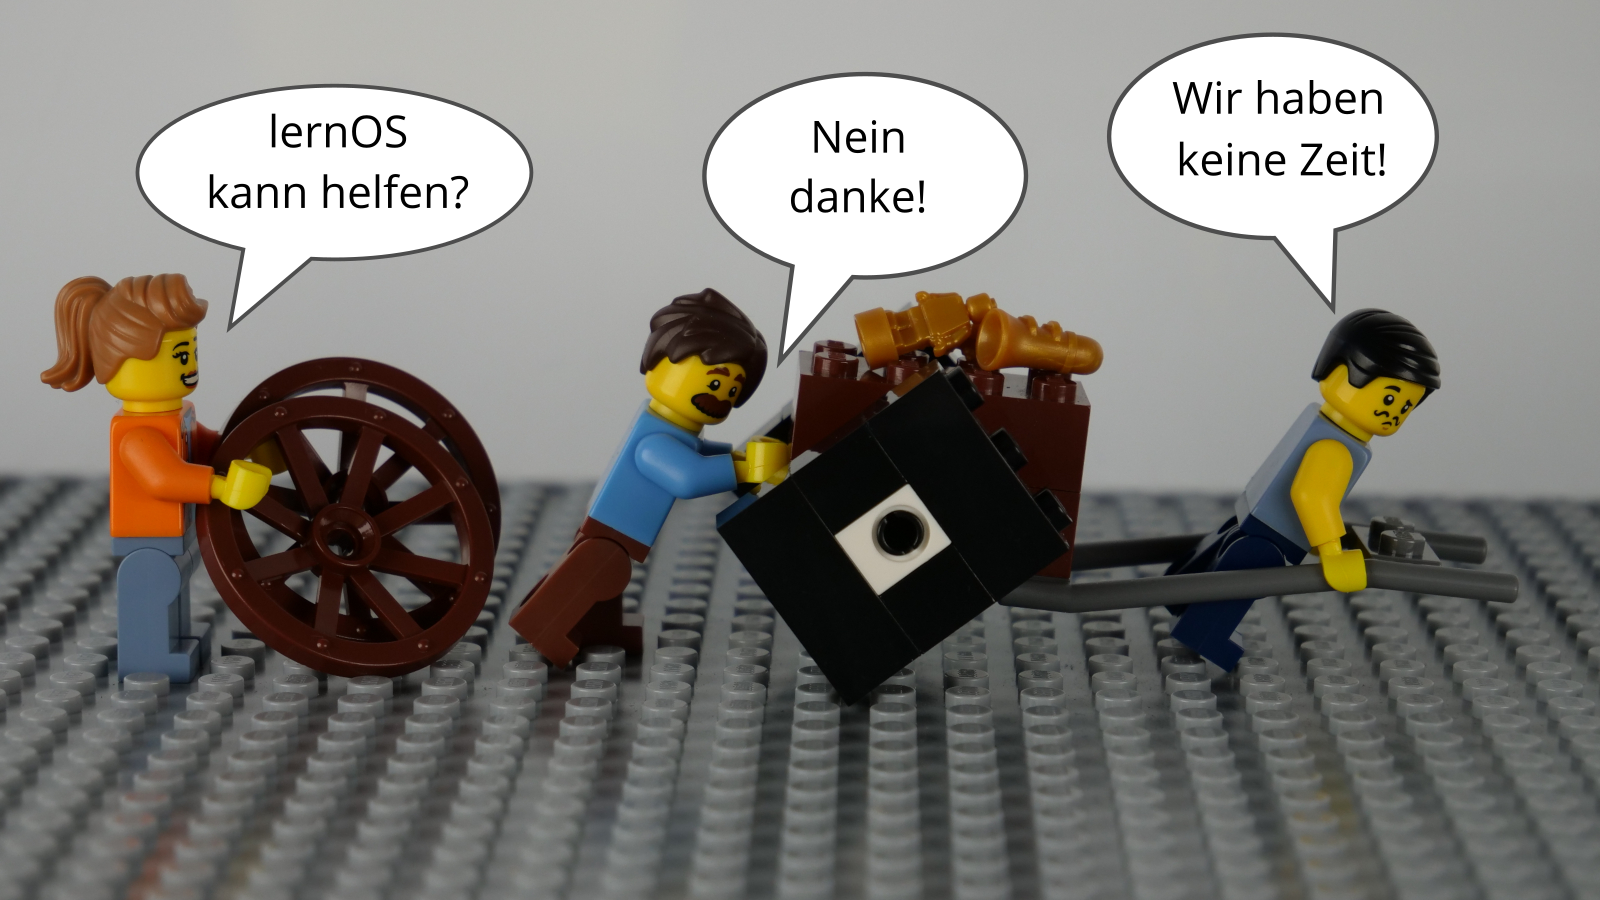
\includegraphics{./tex2pdf.-af94b87e0fdb9aa6/df19bf99afbb44721e135e9eea2ed49ab82560e2.png}
\caption{lernOS Wheel People}
\end{figure}

Bei der Anwendung neuer Handlungsweisen im Privatleben, in der Schule
oder in der Arbeit geht es nicht nur um die Verwendung digitaler Tools.
Um von ``quadratischen Rädern'' auf ``runde Räder'' umzusteigen, musst
Du auch deine Einstellung, deine Werte und deine Fähigkeiten in die
Überlegungen einbeziehen. lernOS nennt diese drei Dimensionen Mindset,
Skillset und Toolset. Sich nur auf ein oder zwei Dimensionen zu
konzentrieren, kann schon helfen. Doch für die besten Ergebnisse sollten
alle drei Dimensionen im persönlichen Entwicklungsprozess berücksichtigt
werden.

\begin{figure}
\centering
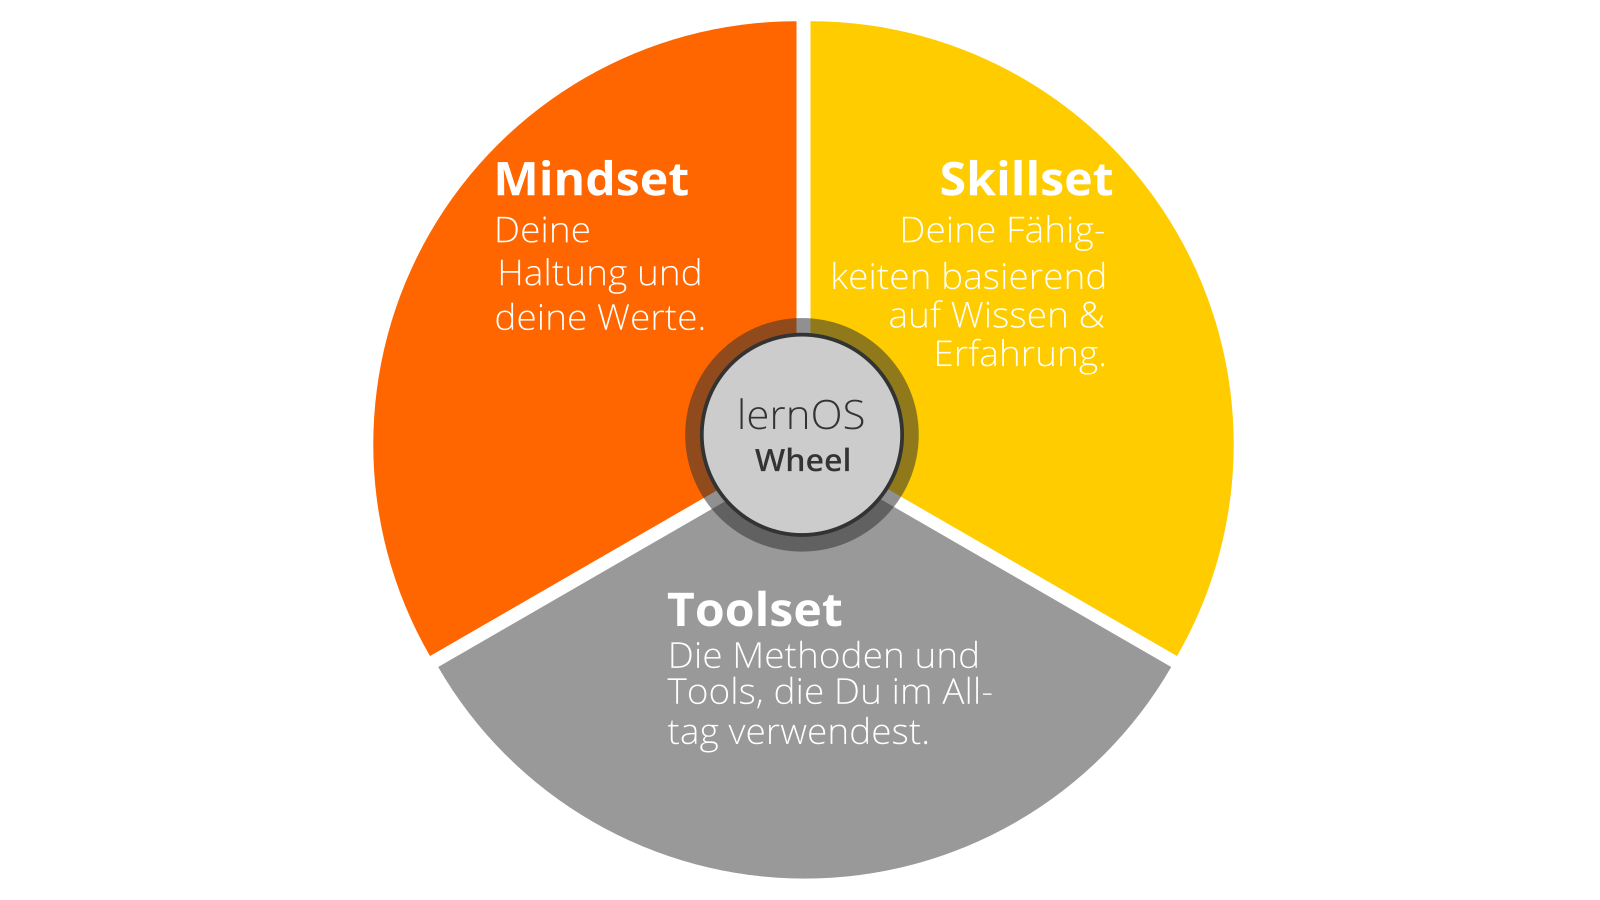
\includegraphics{./tex2pdf.-af94b87e0fdb9aa6/bd77dc0df1ce1b6dae68b830db7f4902bd9b84b4.png}
\caption{lernOS Wheel}
\end{figure}

\hypertarget{mindset-deine-haltung-und-werte}{%
\subsubsection{Mindset: Deine Haltung und
Werte}\label{mindset-deine-haltung-und-werte}}

Das Mindset kann die Haltung und Werte beschrieben werden, die zu
Handlungen und sichtbaren Ergebnissen führen. Diese entwickeln sich im
Laufe der Zeit und bilden die Kultur von Organisationen und der
Gesellschaft. Wenn wir in der Welt handeln, bekommen wir Feedback und
lernen daraus. Im Laufe der Zeit erzeugen wir mentale Modelle der Welt
und Werte, die unser zukünftiges Handeln leiten
(\href{https://www.rrojasdatabank.info/thermo/20388.pdf}{Boisot, 2004}).
Für den Erfolg in der VUCA-Welt sind diese fünf Werte besonders wichtig
(Buhse 2014 \& Petry, 2014):

\begin{enumerate}
\def\labelenumi{\arabic{enumi}.}
\tightlist
\item
  \textbf{Vernetzung} vor Isolation
\item
  \textbf{Vertrauen} vor Misstrauen
\item
  \textbf{Offenheit} vor Silos
\item
  \textbf{Partizipation} vor Ausgrenzung
\item
  \textbf{Agilität} vor Stabilität
\end{enumerate}

Es gibt keine Reihenfolge in den oben genannten Werten, aber für mich
persönlich ist die
\href{https://en.wikipedia.org/wiki/Openness}{Offenheit} der zentrale
Wert für das Mindset des 21. Jahrhunderts. Damit ist die Offenheit für
neue Erfahrungen, Wissen und Ideen, aber auch das offene Teilen von
Wissen, Ideen und Inhalten gemeint (s.a.
\href{https://opendefinition.org}{Definition von Offen}). Du solltest im
Lauf der Zeit ein ``Open First Mindset'' entwickeln, wie im
\href{http://innovationsbeirat.de/open-first}{Open First Manifest}
beschrieben:

\begin{figure}
\centering
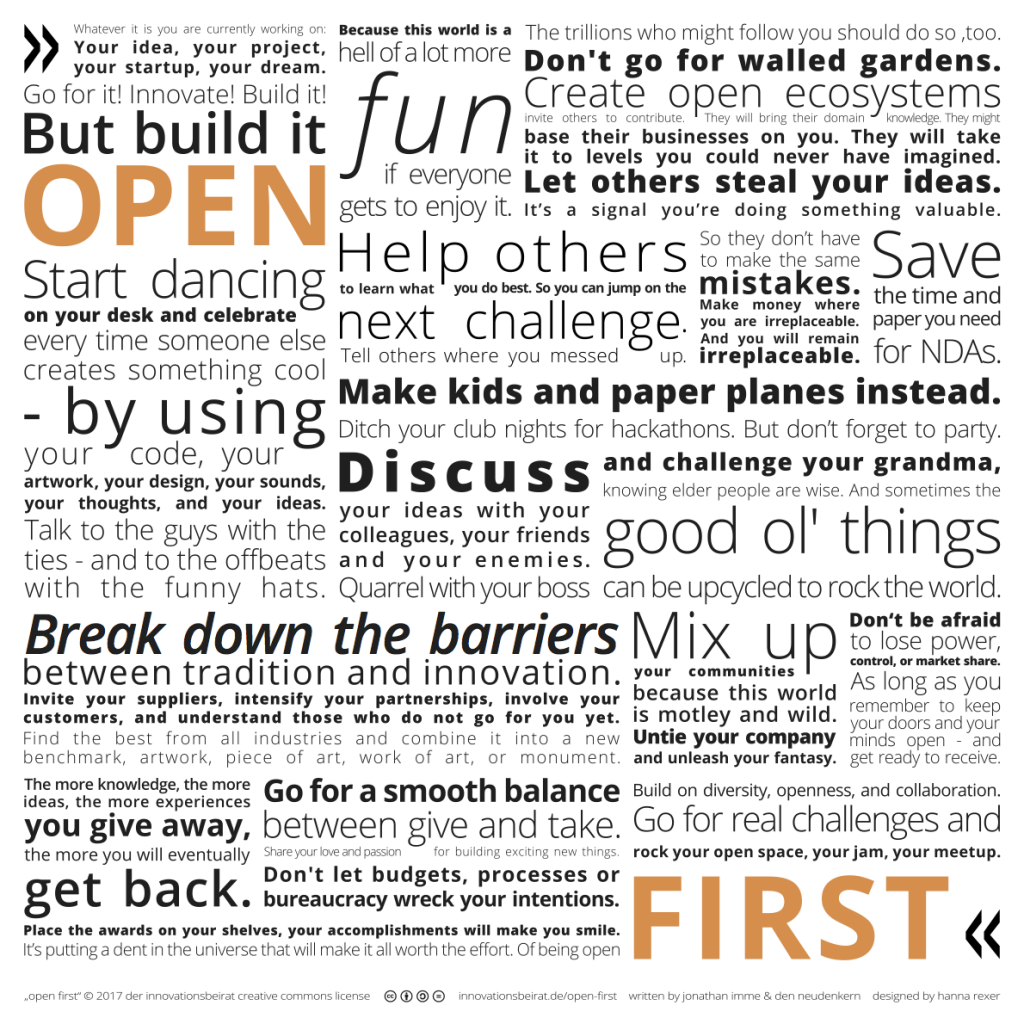
\includegraphics{./tex2pdf.-af94b87e0fdb9aa6/18770edc2ff369daeebec9453c72ff40587e97ed.png}
\caption{Open First Manifesto}
\end{figure}

\textbf{ProTip:} Dein Mindset ist nicht in den sprichwörtlichen Stein
gemeißelt, es kann sich mit der Zeit verändern. Schaue dir das Video
\href{https://www.youtube.com/watch?v=hiiEeMN7vbQ}{Developing a Growth
Mindset} von Carol Dweck an, um mehr darüber zu erfahren.

\hypertarget{skillset-deine-fuxe4higkeiten}{%
\subsubsection{Skillset: Deine
Fähigkeiten}\label{skillset-deine-fuxe4higkeiten}}

Seit den 1980er Jahren sind Fähigkeiten, wie das Lösen von Problemen und
der Austausch mit anderen, für den eigenen Erfolg am wichtigsten. Dazu
gehören insbesondere Fähigkeiten, die in Zukunft nicht einfach durch
Automatisierung und künstliche Intelligenz ersetzt werden können. Um fit
für das 21. Jahrhundert zu werden, solltest du folgende fünf
Fähigkeitsbereiche trainieren
(\href{http://www.p21.org/our-work/p21-framework}{Framework for 21st
Century Learning},
\href{https://ec.europa.eu/jrc/en/publication/eur-scientific-and-technical-research-reports/digcomp-21-digital-competence-framework-citizens-eight-proficiency-levels-and-examples-use}{DigiComp
2.1 Framework}):

\begin{figure}
\centering
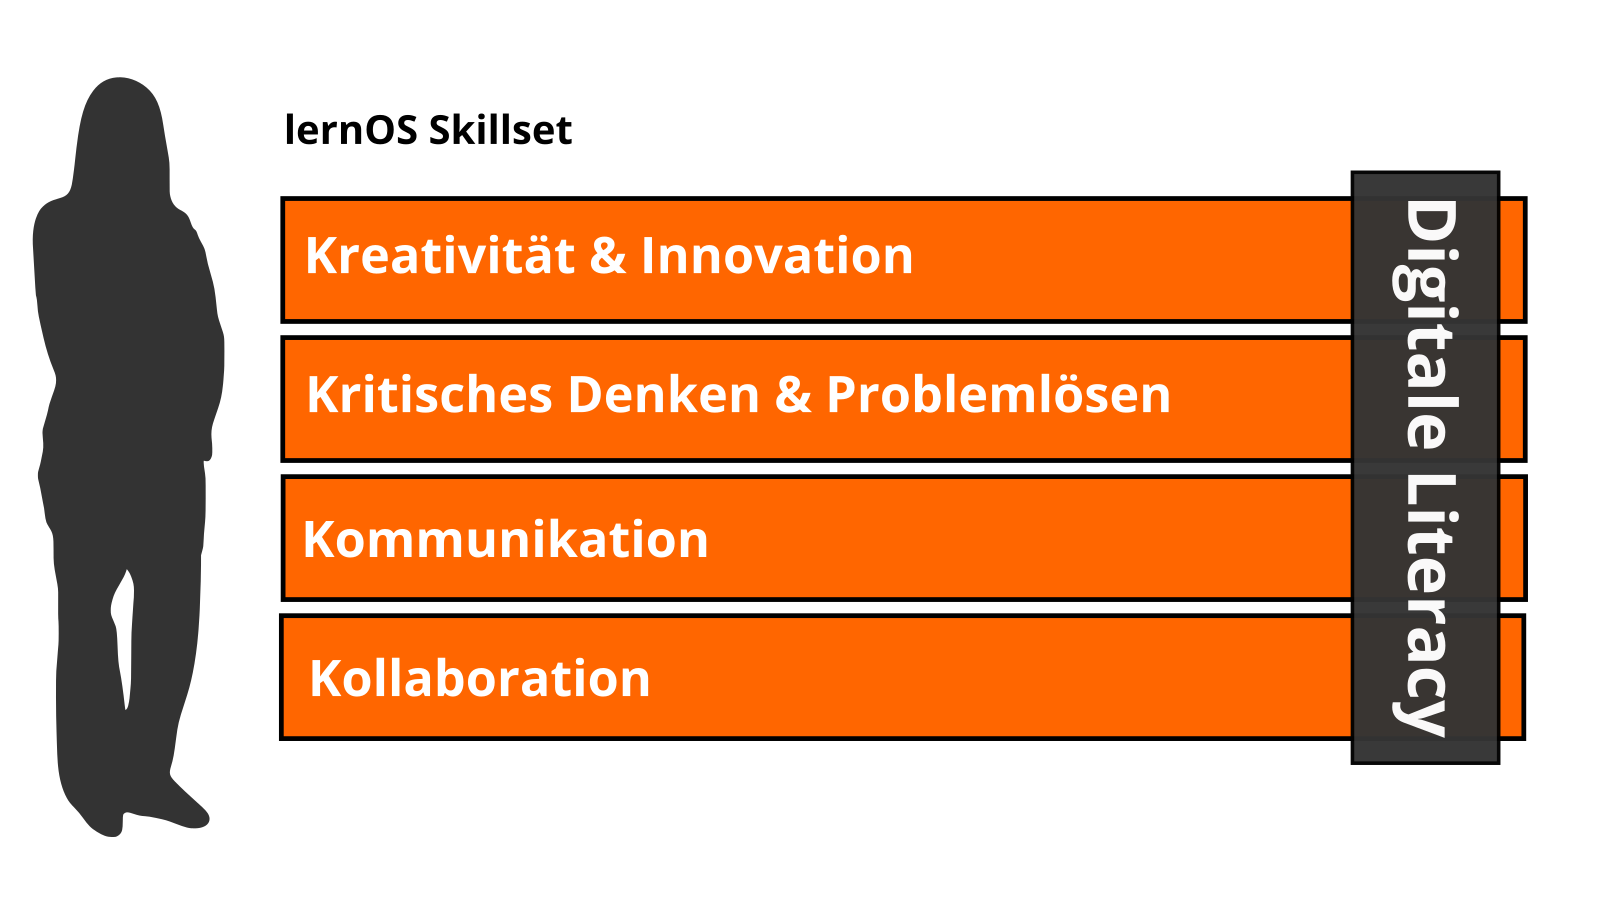
\includegraphics{./tex2pdf.-af94b87e0fdb9aa6/0b6da1ca1544dc3dc47d47c304963015ed6dcf34.png}
\caption{lernOS Skillset}
\end{figure}

Du kannst die folgende Tabelle für eine Selbsteinschätzung am Anfang
eines Learning Sprints nutzen. Wir nutzen die Stufen 1-5 aus dem
\href{https://en.wikipedia.org/wiki/Dreyfus_model_of_skill_acquisition}{Dreyfus
Model of Skill Acquisition} (1 = Novize, 2 = Fortgeschrittener Anfänger,
3 = Kompetent, 4 = Profi, 5 = Experte). Trage deine aktuelle Stufe in
die Spalte ``Ist'' und deine angestrebte Stufe in die Spalte ``Soll''.
Auf der Basis kannst du den Fokus für deine Lernaktivitäten bestimmen.

\begin{longtable}[]{@{}lll@{}}
\toprule
\begin{minipage}[b]{0.72\columnwidth}\raggedright
Fähigkeit\strut
\end{minipage} & \begin{minipage}[b]{0.10\columnwidth}\raggedright
Ist\strut
\end{minipage} & \begin{minipage}[b]{0.10\columnwidth}\raggedright
Soll\strut
\end{minipage}\tabularnewline
\midrule
\endhead
\begin{minipage}[t]{0.72\columnwidth}\raggedright
\textbf{Kreativität \& Innovation}\strut
\end{minipage} & \begin{minipage}[t]{0.10\columnwidth}\raggedright
\strut
\end{minipage} & \begin{minipage}[t]{0.10\columnwidth}\raggedright
\strut
\end{minipage}\tabularnewline
\begin{minipage}[t]{0.72\columnwidth}\raggedright
Kreativ denken\strut
\end{minipage} & \begin{minipage}[t]{0.10\columnwidth}\raggedright
\strut
\end{minipage} & \begin{minipage}[t]{0.10\columnwidth}\raggedright
\strut
\end{minipage}\tabularnewline
\begin{minipage}[t]{0.72\columnwidth}\raggedright
Kreativ mit anderen arbeiten\strut
\end{minipage} & \begin{minipage}[t]{0.10\columnwidth}\raggedright
\strut
\end{minipage} & \begin{minipage}[t]{0.10\columnwidth}\raggedright
\strut
\end{minipage}\tabularnewline
\begin{minipage}[t]{0.72\columnwidth}\raggedright
Innovationen umsetzen\strut
\end{minipage} & \begin{minipage}[t]{0.10\columnwidth}\raggedright
\strut
\end{minipage} & \begin{minipage}[t]{0.10\columnwidth}\raggedright
\strut
\end{minipage}\tabularnewline
\begin{minipage}[t]{0.72\columnwidth}\raggedright
\textbf{Kritisches Denken \& Problemlösen}\strut
\end{minipage} & \begin{minipage}[t]{0.10\columnwidth}\raggedright
\strut
\end{minipage} & \begin{minipage}[t]{0.10\columnwidth}\raggedright
\strut
\end{minipage}\tabularnewline
\begin{minipage}[t]{0.72\columnwidth}\raggedright
Ermittlung von Bedürfnissen und technologischen Möglichkeiten\strut
\end{minipage} & \begin{minipage}[t]{0.10\columnwidth}\raggedright
\strut
\end{minipage} & \begin{minipage}[t]{0.10\columnwidth}\raggedright
\strut
\end{minipage}\tabularnewline
\begin{minipage}[t]{0.72\columnwidth}\raggedright
Dingen effektiv auf den Grund gehen\strut
\end{minipage} & \begin{minipage}[t]{0.10\columnwidth}\raggedright
\strut
\end{minipage} & \begin{minipage}[t]{0.10\columnwidth}\raggedright
\strut
\end{minipage}\tabularnewline
\begin{minipage}[t]{0.72\columnwidth}\raggedright
Urteile und Entscheidungen treffen\strut
\end{minipage} & \begin{minipage}[t]{0.10\columnwidth}\raggedright
\strut
\end{minipage} & \begin{minipage}[t]{0.10\columnwidth}\raggedright
\strut
\end{minipage}\tabularnewline
\begin{minipage}[t]{0.72\columnwidth}\raggedright
Technische und nicht-technische Probleme lösen\strut
\end{minipage} & \begin{minipage}[t]{0.10\columnwidth}\raggedright
\strut
\end{minipage} & \begin{minipage}[t]{0.10\columnwidth}\raggedright
\strut
\end{minipage}\tabularnewline
\begin{minipage}[t]{0.72\columnwidth}\raggedright
Kreativ Technologien zur Lösung von Problemen einsetzen\strut
\end{minipage} & \begin{minipage}[t]{0.10\columnwidth}\raggedright
\strut
\end{minipage} & \begin{minipage}[t]{0.10\columnwidth}\raggedright
\strut
\end{minipage}\tabularnewline
\begin{minipage}[t]{0.72\columnwidth}\raggedright
\textbf{Kommunikation}\strut
\end{minipage} & \begin{minipage}[t]{0.10\columnwidth}\raggedright
\strut
\end{minipage} & \begin{minipage}[t]{0.10\columnwidth}\raggedright
\strut
\end{minipage}\tabularnewline
\begin{minipage}[t]{0.72\columnwidth}\raggedright
Gedanken und Ideen klar und effektiv artikulieren\strut
\end{minipage} & \begin{minipage}[t]{0.10\columnwidth}\raggedright
\strut
\end{minipage} & \begin{minipage}[t]{0.10\columnwidth}\raggedright
\strut
\end{minipage}\tabularnewline
\begin{minipage}[t]{0.72\columnwidth}\raggedright
Effektiv zuhören und Bedeutung erkennen\strut
\end{minipage} & \begin{minipage}[t]{0.10\columnwidth}\raggedright
\strut
\end{minipage} & \begin{minipage}[t]{0.10\columnwidth}\raggedright
\strut
\end{minipage}\tabularnewline
\begin{minipage}[t]{0.72\columnwidth}\raggedright
Kommunikation nutzen, um zu informieren, zu unterrichten, zu motivieren
und zu überzeugen\strut
\end{minipage} & \begin{minipage}[t]{0.10\columnwidth}\raggedright
\strut
\end{minipage} & \begin{minipage}[t]{0.10\columnwidth}\raggedright
\strut
\end{minipage}\tabularnewline
\begin{minipage}[t]{0.72\columnwidth}\raggedright
Vielfältige Medien und Technologien nutzen\strut
\end{minipage} & \begin{minipage}[t]{0.10\columnwidth}\raggedright
\strut
\end{minipage} & \begin{minipage}[t]{0.10\columnwidth}\raggedright
\strut
\end{minipage}\tabularnewline
\begin{minipage}[t]{0.72\columnwidth}\raggedright
Effektiv in verschiedenen Umgebungen kommunizieren\strut
\end{minipage} & \begin{minipage}[t]{0.10\columnwidth}\raggedright
\strut
\end{minipage} & \begin{minipage}[t]{0.10\columnwidth}\raggedright
\strut
\end{minipage}\tabularnewline
\begin{minipage}[t]{0.72\columnwidth}\raggedright
\textbf{Kollaboration}\strut
\end{minipage} & \begin{minipage}[t]{0.10\columnwidth}\raggedright
\strut
\end{minipage} & \begin{minipage}[t]{0.10\columnwidth}\raggedright
\strut
\end{minipage}\tabularnewline
\begin{minipage}[t]{0.72\columnwidth}\raggedright
Effektiv und respektvoll in gemischten Teams arbeiten\strut
\end{minipage} & \begin{minipage}[t]{0.10\columnwidth}\raggedright
\strut
\end{minipage} & \begin{minipage}[t]{0.10\columnwidth}\raggedright
\strut
\end{minipage}\tabularnewline
\begin{minipage}[t]{0.72\columnwidth}\raggedright
Flexibilität und Bereitschaft zeigen sowie bei notwendigen Kompromissen
unterstützen, um ein gemeinsames Ziel zu erreichen\strut
\end{minipage} & \begin{minipage}[t]{0.10\columnwidth}\raggedright
\strut
\end{minipage} & \begin{minipage}[t]{0.10\columnwidth}\raggedright
\strut
\end{minipage}\tabularnewline
\begin{minipage}[t]{0.72\columnwidth}\raggedright
Verantwortung für die gemeinsame Arbeit übernehmen und einzelne Beiträge
wertschätzen\strut
\end{minipage} & \begin{minipage}[t]{0.10\columnwidth}\raggedright
\strut
\end{minipage} & \begin{minipage}[t]{0.10\columnwidth}\raggedright
\strut
\end{minipage}\tabularnewline
\begin{minipage}[t]{0.72\columnwidth}\raggedright
Mit digitalen Medien interagieren, sich beteiligen, austauschen und
zusammenarbeiten\strut
\end{minipage} & \begin{minipage}[t]{0.10\columnwidth}\raggedright
\strut
\end{minipage} & \begin{minipage}[t]{0.10\columnwidth}\raggedright
\strut
\end{minipage}\tabularnewline
\begin{minipage}[t]{0.72\columnwidth}\raggedright
Digitale Identität verwalten\strut
\end{minipage} & \begin{minipage}[t]{0.10\columnwidth}\raggedright
\strut
\end{minipage} & \begin{minipage}[t]{0.10\columnwidth}\raggedright
\strut
\end{minipage}\tabularnewline
\begin{minipage}[t]{0.72\columnwidth}\raggedright
\textbf{Digital Literacy}\strut
\end{minipage} & \begin{minipage}[t]{0.10\columnwidth}\raggedright
\strut
\end{minipage} & \begin{minipage}[t]{0.10\columnwidth}\raggedright
\strut
\end{minipage}\tabularnewline
\begin{minipage}[t]{0.72\columnwidth}\raggedright
Surfen, suchen, Daten, Informationen und digitale Inhalte filtern\strut
\end{minipage} & \begin{minipage}[t]{0.10\columnwidth}\raggedright
\strut
\end{minipage} & \begin{minipage}[t]{0.10\columnwidth}\raggedright
\strut
\end{minipage}\tabularnewline
\begin{minipage}[t]{0.72\columnwidth}\raggedright
Auswertung und Verwaltung von Daten, Informationen und digitalen
Inhalten\strut
\end{minipage} & \begin{minipage}[t]{0.10\columnwidth}\raggedright
\strut
\end{minipage} & \begin{minipage}[t]{0.10\columnwidth}\raggedright
\strut
\end{minipage}\tabularnewline
\begin{minipage}[t]{0.72\columnwidth}\raggedright
Schutz digitaler Geräte und personenbezogener Daten\strut
\end{minipage} & \begin{minipage}[t]{0.10\columnwidth}\raggedright
\strut
\end{minipage} & \begin{minipage}[t]{0.10\columnwidth}\raggedright
\strut
\end{minipage}\tabularnewline
\begin{minipage}[t]{0.72\columnwidth}\raggedright
Entwicklung, Integration und Überarbeitung digitaler Inhalte\strut
\end{minipage} & \begin{minipage}[t]{0.10\columnwidth}\raggedright
\strut
\end{minipage} & \begin{minipage}[t]{0.10\columnwidth}\raggedright
\strut
\end{minipage}\tabularnewline
\begin{minipage}[t]{0.72\columnwidth}\raggedright
Umgang mit Urheberrechten und Lizenzen\strut
\end{minipage} & \begin{minipage}[t]{0.10\columnwidth}\raggedright
\strut
\end{minipage} & \begin{minipage}[t]{0.10\columnwidth}\raggedright
\strut
\end{minipage}\tabularnewline
\begin{minipage}[t]{0.72\columnwidth}\raggedright
Programmieren, Scripten und Kodieren\strut
\end{minipage} & \begin{minipage}[t]{0.10\columnwidth}\raggedright
\strut
\end{minipage} & \begin{minipage}[t]{0.10\columnwidth}\raggedright
\strut
\end{minipage}\tabularnewline
\bottomrule
\end{longtable}

\textbf{ProTip:} Das Mozilla
\href{https://learning.mozilla.org/en-US/web-literacy}{Web Literacy
Framework} bietet Übungen zu Digital Literacy und Fähigkeiten des 21.
Jahrhunderts.

\hypertarget{toolset-digitale-tools-die-du-verwendest}{%
\subsubsection{Toolset: Digitale Tools, die du
verwendest}\label{toolset-digitale-tools-die-du-verwendest}}

Das
\href{https://www.oreilly.com/pub/a/web2/archive/what-is-web-20.html}{Web
2.0} und die sozialen Medien gibt es seit 2005. Nicht jeder muss alle
digitalen Tools kennen, aber man sollte einen Überblick haben, die
Prinzipien kennen und die richtigen Tools für sich auswählen. Das
Conversation Prism gibt einen guten Überblick über heute verfügbare Web
2.0 Plattformen:

\begin{figure}
\centering
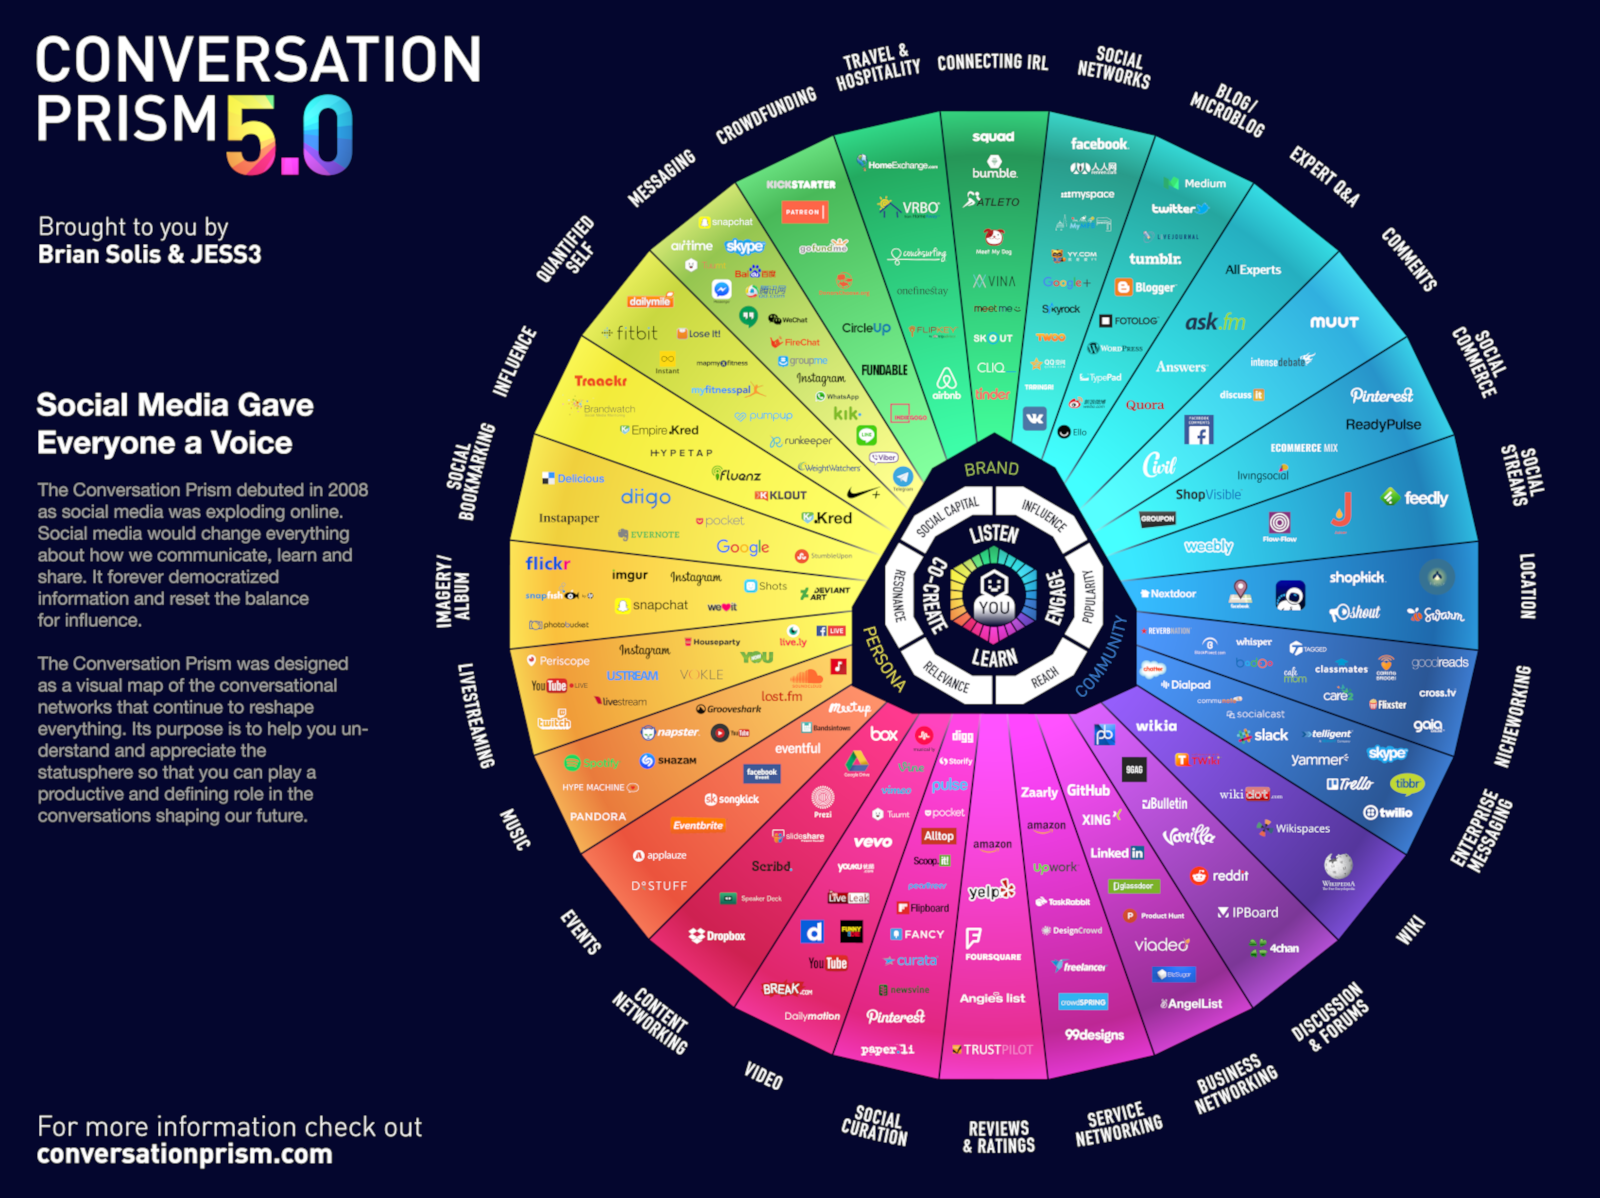
\includegraphics{./tex2pdf.-af94b87e0fdb9aa6/6b3c3be66bbf7be83f482f370fe8c95d5cbaa199.png}
\caption{Conversation Prism 5.0 (conversationprism.com) von Brian Solis
und JESS3}
\end{figure}

Für Einsteiger können 28 Kategorien und Dutzende von Tools überwältigend
sein. Die folgende Liste gibt daher einen Überblick über die für lernOS
wichtigsten Tools:

\begin{enumerate}
\def\labelenumi{\arabic{enumi}.}
\tightlist
\item
  \textbf{Office- \& Produktivität}, z.B. Dropbox, Evernote, FreeMind, G
  Suite, MindManager, Office 365, OneNote, SharePoint, Trello, XMind
\item
  \textbf{Chat \& Messenger}, z.B. Google Hangouts Chat, Mattermost,
  Microsoft Teams, Rocketchat, Slack, Telegram, Threema, WeChat,
  WhatsApp
\item
  \textbf{Soziale Netwerke}, z.B. IBM Connections, Jive, LinkedIn,
  Mastodon, Twitter, Workplace by Facebook, Xing, Yammer
\item
  \textbf{Videokonferenz}, z.B. Google Hangouts Meet, GoToMeeting,
  Microsoft Teams, Skype, Skype for Business, WebEx, Zoom
\item
  \textbf{Weblogs \& Wikis}, z.B. Confluence, DokuWiki, LinkedIn
  (Artikel), MediaWiki, Medium, Tumblr, Wikipedia, WordPress
\end{enumerate}

\textbf{ProTip:} Das
\href{https://github.com/cogneon/lernos-core/wiki}{lernOS Wiki} enthält
eine Linkliste zu allen genannten Tools. In Zukunft wird es dort auch
Tutorials zur Nutzung der Tools geben.

\hypertarget{lernos-circle-die-macht-von-peer-support}{%
\subsection{lernOS Circle: Die Macht von ``Peer
Support''}\label{lernos-circle-die-macht-von-peer-support}}

Wenn du lernOS nicht alleine praktizieren möchtest, kannst du Dich in
einer Gruppe von 4-5 Personen, die Learning Circle genannt wird,
zusammenschließen. Ein Circle ist eine
\href{https://en.wikipedia.org/wiki/Peer_support}{Peer Support} Gruppe,
in der sich die Mitglieder gegenseitig mit Feedback, Erfahrung, Wissen
und Reflexion helfen. Der Circle ist ein ``Kreis des Vertrauens'': was
im Circle passiert, bleibt im Circle! Die Circle-Mitglieder treffen sich
wöchentlich und folgen dabei einem vorgegebenen Ablauf, der den Lern-
und Entwicklungsprozess strukturiert.

\begin{figure}
\centering
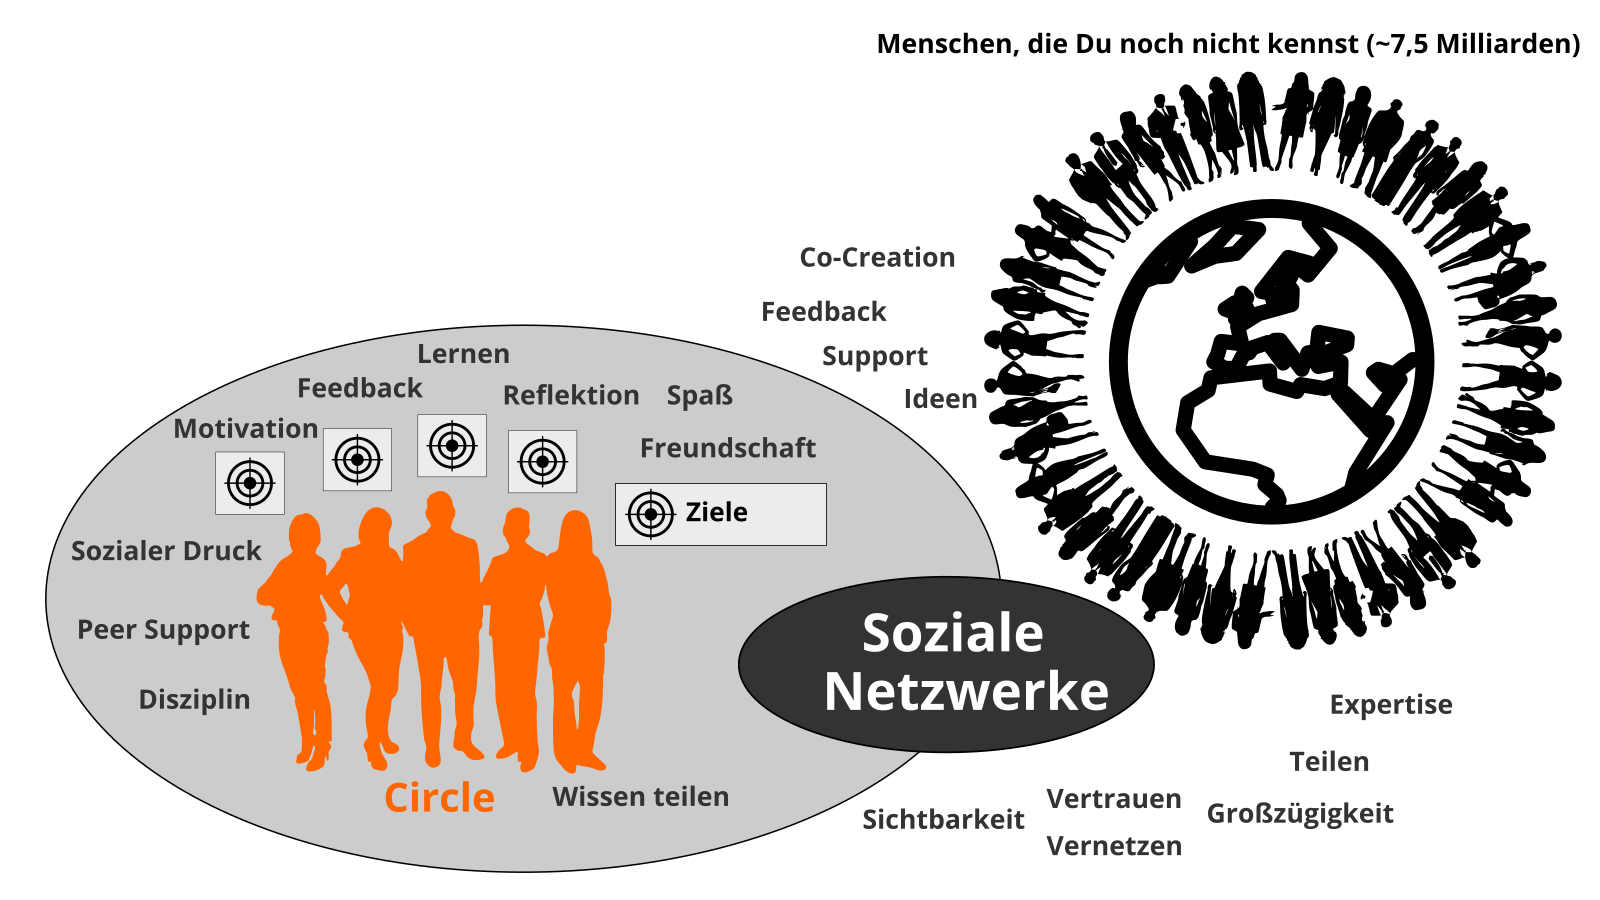
\includegraphics{./tex2pdf.-af94b87e0fdb9aa6/0d67e1021e5c580615fa48b0a1dfe050338091a7.png}
\caption{Learning Circle}
\end{figure}

Einmal pro Woche trifft sich der Learning Circle. Jedes Treffen folgt
einem vorgegebenen Ablauf (siehe Anhang) mit einem Check-in, Übungen
(Katas) und einem Check-out. Der Zeitraum für das Weekly kann an die
Bedürfnisse der Circle-Mitglieder angepasst werden. Der vorgeschlagene
Zeitraum ist Freitag zwischen 11-12 Uhr.

\textbf{ProTip:} Kata ist anderes Wort für Übung. Es kommt aus dem
Bereich des Erlernens von Programmier-Fähigkeiten im
Peer-Learning-Format. Lies mehr über dieses Format unter
\href{http://codekata.com}{codekata.com}.

Das Weekly kann als persönliches Treffen (face-2-face) oder virtuell
stattfinden. Der Circle muss Tools für die Kommunikation und
Dokumentation zwischen den Treffen definieren. Die folgenden Anwendungen
haben sich in der Praxis bewährt:

\begin{itemize}
\tightlist
\item
  Microsoft Teams
\item
  OneNote
\item
  SharePoint
\item
  Skype
\item
  Skype for Business
\item
  Slack
\item
  WebEx
\item
  WhatsApp
\item
  Yammer
\item
  Zoom
\end{itemize}

Wenn du in deiner Organisation ein Enterprise Social Network (ESN) wie
z.B. Jive oder Connections hast, kann das für die Unterstützung von
lernOS Circles auch eine gute Option sein.

\textbf{ProTip:} Wählt für möglichst einfache Benutzbarkeit ein Tool,
das Kommunikation und Dokumentation gleichzeitig unterstützt, z.B.
\href{https://products.office.com/en-us/microsoft-teams/group-chat-software}{Microsoft
Teams}. In Microsoft Teams könnt Ihr den Kanal ``Allgemein'' für
Kommunikation, die Audio-/Video-Konferenz-Funktion für virtuelle
Meetings und ein OneNote-Notizbuch zur Dokumentation nutzen.

\hypertarget{lernpfade-fuxfcr-einsteigerinnen-noobs}{%
\section{Lernpfade für Einsteiger*innen
(NOOBs)}\label{lernpfade-fuxfcr-einsteigerinnen-noobs}}

Ein lernOS Lernpfad ist eine Zusammenstellung von Übungen (Katas), mit
denen du neue Fähigkeiten erlernst und im Lauf der Zeit eine neue
Haltung entwickelst. Ein Lernpfad kann innerhalb eines lernOS Sprints
durchlaufen werden. lernOS Einsteiger*innen (NOOBs) können aus einem von
drei Lernpfaden wählen:

\begin{figure}
\centering
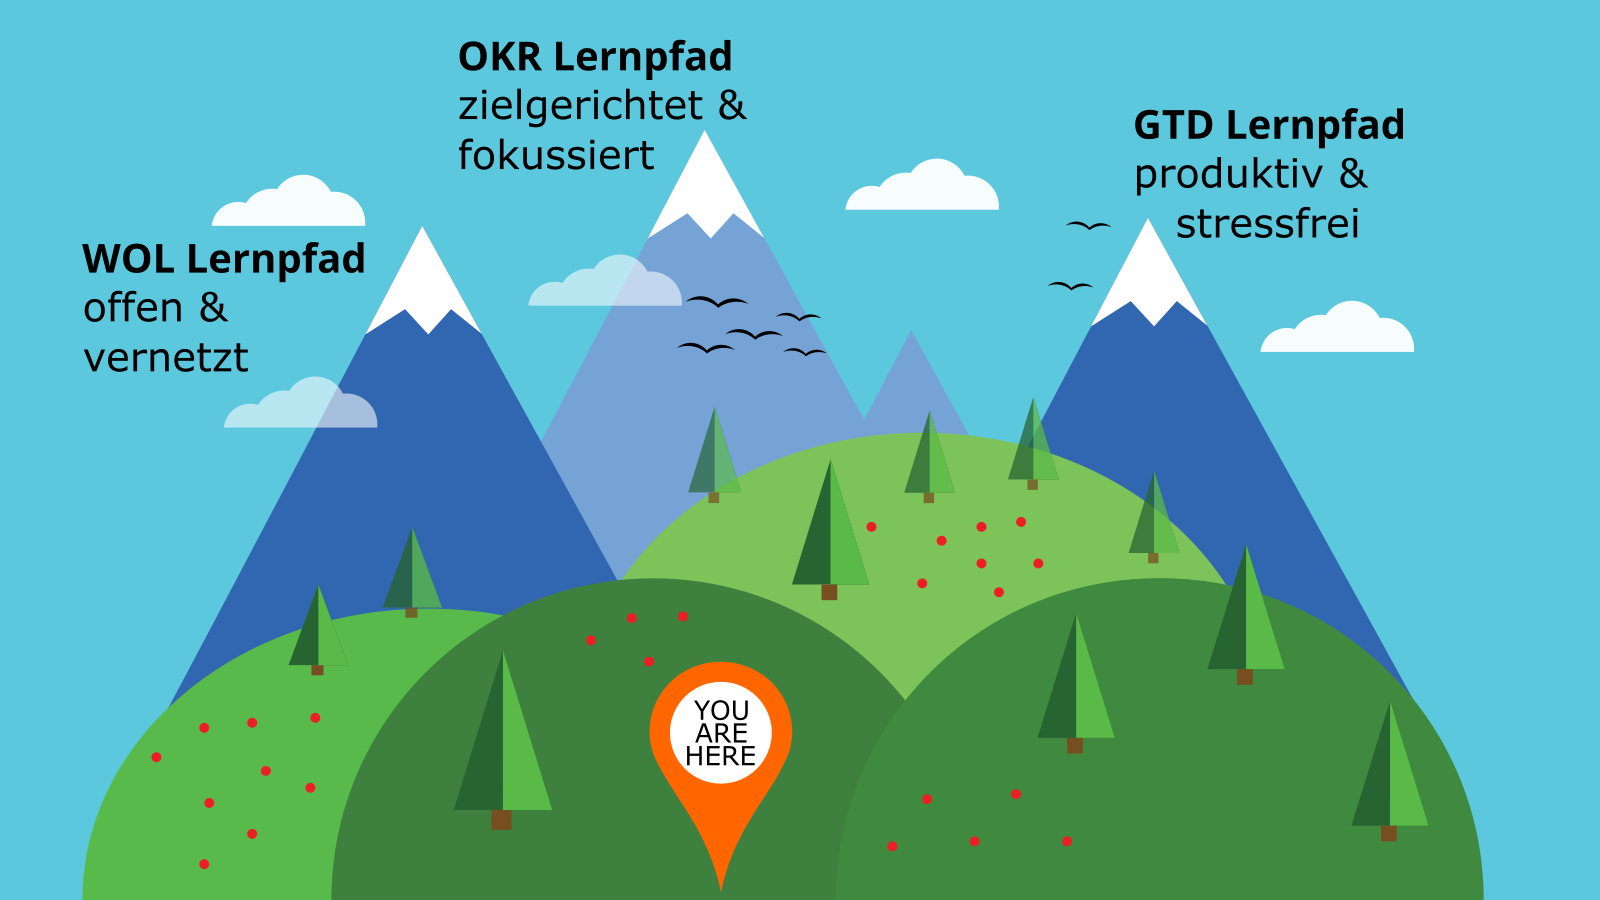
\includegraphics{./tex2pdf.-af94b87e0fdb9aa6/c587d0e577abadd8b4876e8bdf99260f63e71cf7.png}
\caption{lernOS Lernpfade für Einsteiger*innen}
\end{figure}

\begin{enumerate}
\def\labelenumi{\arabic{enumi}.}
\tightlist
\item
  \textbf{WOL Lernpfad:} in diesem Lernpfad lernst du, \textbf{offen}
  und \textbf{vernetzt} zu Arbeiten, sowie deine Ergebnisse sichtbar zu
  machen und darüber zu erzählen. Der Lernpfad basiert auf den
  \href{https://workingoutloud.com/de/circle-guides}{Working Out Loud
  Circle Guides} von John Stepper.
\item
  \textbf{OKR Lernpfad:} dieser Lernpfad hilft dir,
  \textbf{zielgerichtet} und \textbf{fokussiert} zu Arbeiten und zu
  Lernen. Dabei geht es nicht nur um alltägliche Ziele, sondern auch um
  die großen Ziele in der Arbeit und im Leben (Moonshots). Der Lernpfad
  basiert auf der Methode
  \href{https://rework.withgoogle.com/guides/set-goals-with-okrs/steps/introduction/}{Objectives
  \& Key Results} (OKR) von Google.
\item
  \textbf{GTD Lernpfad:} In diesem Lernpfad lernst du, bei der Fülle von
  Aufgaben \textbf{produktiv} zu sein und in jeder Situation
  \textbf{stressfrei} den Überblick zu behalten. Der Lernpfad basiert
  auf der Methode
  \href{https://gettingthingsdone.com/what-is-gtd/}{Getting Things Done}
  (GTD) von David Allen.
\end{enumerate}

\textbf{ProTip:} für einen Sprint sollte nur einer der drei Lernpfade
gewählt werden. Alle drei Lernpfade können in aufeinanderfolgenden
Sprints durchlaufen werden. Tandems und Circles sollten Lernpfade nicht
mischen, da ihr sonst im Weekly nicht von den Erfahrungen der anderen
profitieren könnt.

\hypertarget{wol-lernpfad}{%
\subsection{WOL Lernpfad}\label{wol-lernpfad}}

Sein Wissen mit anderen offen zu teilen und von dem Wissen anderer zu
profitieren hilft, dass nicht alle das Rad immer wieder neu erfinden
müssen. Gemäß der
\href{https://workingoutloud.com/en/circle-guides}{Working Out Loud
Methode} von John Stepper kannst du, lernen

\begin{enumerate}
\def\labelenumi{\arabic{enumi}.}
\tightlist
\item
  Dir ein eigenes Lernziel für den Sprint zu stecken.
\item
  Menschen und Communities identifizieren, die mit deinem Ziel zu tun
  haben.
\item
  Beiträge veröffentlichen und Wertschätzung zeigen, um dir systematisch
  und zielorientiert ein Netzwerk aufzubauen.
\item
  Die Unterstützung deines neuen Netzwerks nutzen, um deine Ziele
  schneller und einfacher zu erreichen.
\end{enumerate}

Dieser Lernpfad ist eine auf 11 Übungen verkürzte Version der Circle
Methode von John Stepper (31 Übungen). Die Grundidee ``Working Out Loud
= Observable Work + Narrating Your Work''
\href{https://thebryceswrite.com/2010/11/29/when-will-we-work-out-loud-soon/}{von
Bryce Williams} bleibt dabei jedoch erhalten.

\hypertarget{gestalte-dein-future-backwards-kata}{%
\subsubsection{Gestalte dein Future Backwards
(Kata)}\label{gestalte-dein-future-backwards-kata}}

\textbf{Gestalte deine Zukunft durch Reflexion von Gegenwart und
Vergangenheit und den Entwurf einer persönlichen Vision}

\emph{\textbf{Dauer:} 30 Minuten}

Diese Kata basiert auf der Methode
\href{https://cognitive-edge.com/methods/the-future-backwards/}{The
Future, Backwards} von Dave Snowden. Mit der Kata erhält man eine gute
Sicht auf die persönliche Gesamtsituation durch einen Blick in die
Vergangenheit und auf mögliche Zukünfte. Die Perspektive der Kata kann
kurzfristig (1-2 Jahre), mittelfristig (3-5 Jahre) oder langfristig
(ganzes Leben) sein.

\textbf{Anleitung:}

\begin{enumerate}
\def\labelenumi{\arabic{enumi}.}
\tightlist
\item
  Bereite deinen Future Backwards Canvas vor
  (\href{https://cognitive-edge.com/wp-content/uploads/2015/01/3---ChrisFl-IMG-0058-wpcf_300x225.jpg}{Beispiel}).
  Das kann im einfachsten Fall ein Blatt Papier im Querformat mit einem
  um 90 Grad nach rechts gedrehten ``Y'' darauf sein, Das Y stellt die
  aktuelle Situation (current state), die Vergangenheit, die Vision
  (heaven), die Anti-Vision (hell) sowie den ``Stairway to Heaven'' dar.
  Definiere die Zeitspanne, die du in Vergangenheit und Zukunft schauen
  möchtest (kurz-/mittel-/langfristig) (5 Minuten)
\item
  Beschreibe deine aktuelle Situation in in 3-5 kurzen Sätzen (5
  Minuten)
\item
  Beschreibe die 3-5 Schlüssel-Ereignisse in der Vergangenheit, die zur
  aktuellen Situation geführt haben (5 Minuten)
\item
  Beschreibe deine Vision in 3-5 kurzen Sätzen (5 Minuten)
\item
  Beschreibe deine Anti-Vision in 3-5 kurzen Sätzen (5 Minuten)
\item
  Beschreibe die 3-5 Schlüssel-Aktivitäten oder -Projekte, die deine
  Vision Wirklichkeit werden lässt und die Anti-Vision verhindert (5
  Minuten)
\end{enumerate}

\textbf{ProTip:} \href{https://twitter.com/GoodTransfer}{Helmut Hönsch}
hat ein \href{}{LearningSprintBooklet} erstellt, das eine Vorlage für
ein Future Backwards enthält.

\hypertarget{visuell-denken-mit-dem-lernos-canvas-kata}{%
\subsubsection{Visuell denken mit dem lernOS Canvas
(Kata)}\label{visuell-denken-mit-dem-lernos-canvas-kata}}

Ein Canvas ist eine visuelle Struktur, die für die strukturierte
Bearbeitung mehrere Bereiche parallel verwendet werden kann. Auf diese
Weise verwendet man einen Canvas als visuelle Checkliste. Er kann aber
auch für das Erzählen komplexer Geschichten verwendet werden. Die Idee
kam ursprünglich von Alex Osterwalder, der den
\href{https://en.wikipedia.org/wiki/Business_Model_Canvas}{Business
Model Canvas} entwickelt hat. Der lernOS Canvas verwendet die gleiche
Grundstruktur wie der Business Model Canvas. Doch die Benennungen der
Bereiche wurden geändert, um die Arbeitsthemen von lernOS abzudecken.

Der lernOS Canvas kann von der \href{https://lernOS.org}{lernOS
Webseite} in verschiedenen Formaten heruntergeladen (z.B. PowerPoint,
PDF, PNG) werden. Um mit dem Canvas flexibel arbeiten zu können,
solltest du nie darauf schreiben. Aus diesem Grund wurden Haftnotizen
erfunden!

\begin{figure}
\centering
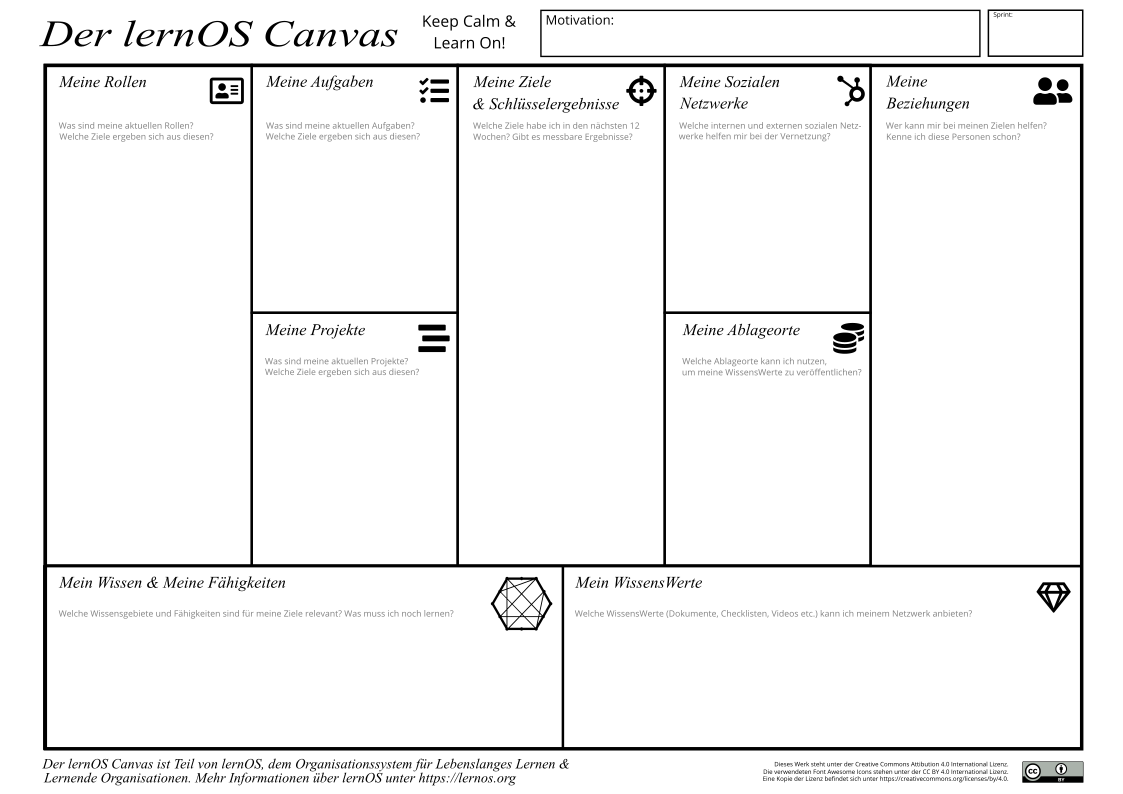
\includegraphics{./tex2pdf.-af94b87e0fdb9aa6/a706e42b1eb1c1bbbe80e1109cff3eb164666bfd.png}
\caption{lernOS Canvas}
\end{figure}

Der obere Teil des Canvas enthält Motivations- oder Mission Statement
(wenn du eines hast) und Nummer oder Datum des Sprints. Im Bereich
``Meine Ziele \& Schlüsselergebnisse'' werden die Ziele für den
aktuellen Sprint dokumentiert. Die Bereiche ``Meine Rollen'', ``Meine
Aktivitäten'', ``Meine Projekte'' und ``Mein Wissen \& Meine
Fähigkeiten'' können genutzt werden, um mögliche Ziele zu
identifizieren. Die Bereiche ``Meine Beziehungen'' und ``Meine Sozialen
Netzwerke'' werden zur Identifikation von Personen verwendet, die bei
der Zielerreichung unterstützen können. Vorhandene Ressourcen (z.B.
Dokumente, Checklisten, Videos etc.) werden in ``Meine WissensWerte''
aufgeführt. Die bei ``Meine Ablageorte'' aufgeführten Ablagen werden
genutzt, um wertvolle Ressourcen großzügig mit dem Netzwerk zu teilen.

\hypertarget{lege-dein-ziel-fuxfcr-die-nuxe4chsten-12-wochen-fest-kata-1}{%
\subsubsection{Lege dein Ziel für die nächsten 12 Wochen fest (Kata
1)}\label{lege-dein-ziel-fuxfcr-die-nuxe4chsten-12-wochen-fest-kata-1}}

In dieser Kata wählst Du Dein Ziel für den Sprint. Das Ziel kann bis zur
4. Woche verfeinert werden, aber nicht danach.

\textbf{Übung (25 Minuten):}

Was willst du in den nächsten zwölf Wochen erreichen? Wähle ein Ziel,
das Dich wirklich, wirklich wichtig ist und bei dem du im Sprint
Fortschritte machen kannst. du wirst die die OKR-Methode von Google
verwenden, um dieses Ziel zu definieren. Für den NOOB Pfad ist es nicht
erste Priorität, das Ziel zu erreichen. Im Fokus steht zu lernen, wie du
mit Hilfe eines offenen Arbeitsstils und der Entwicklung eines Netzwerks
Ziele einfacher erreichst.

\begin{figure}
\centering
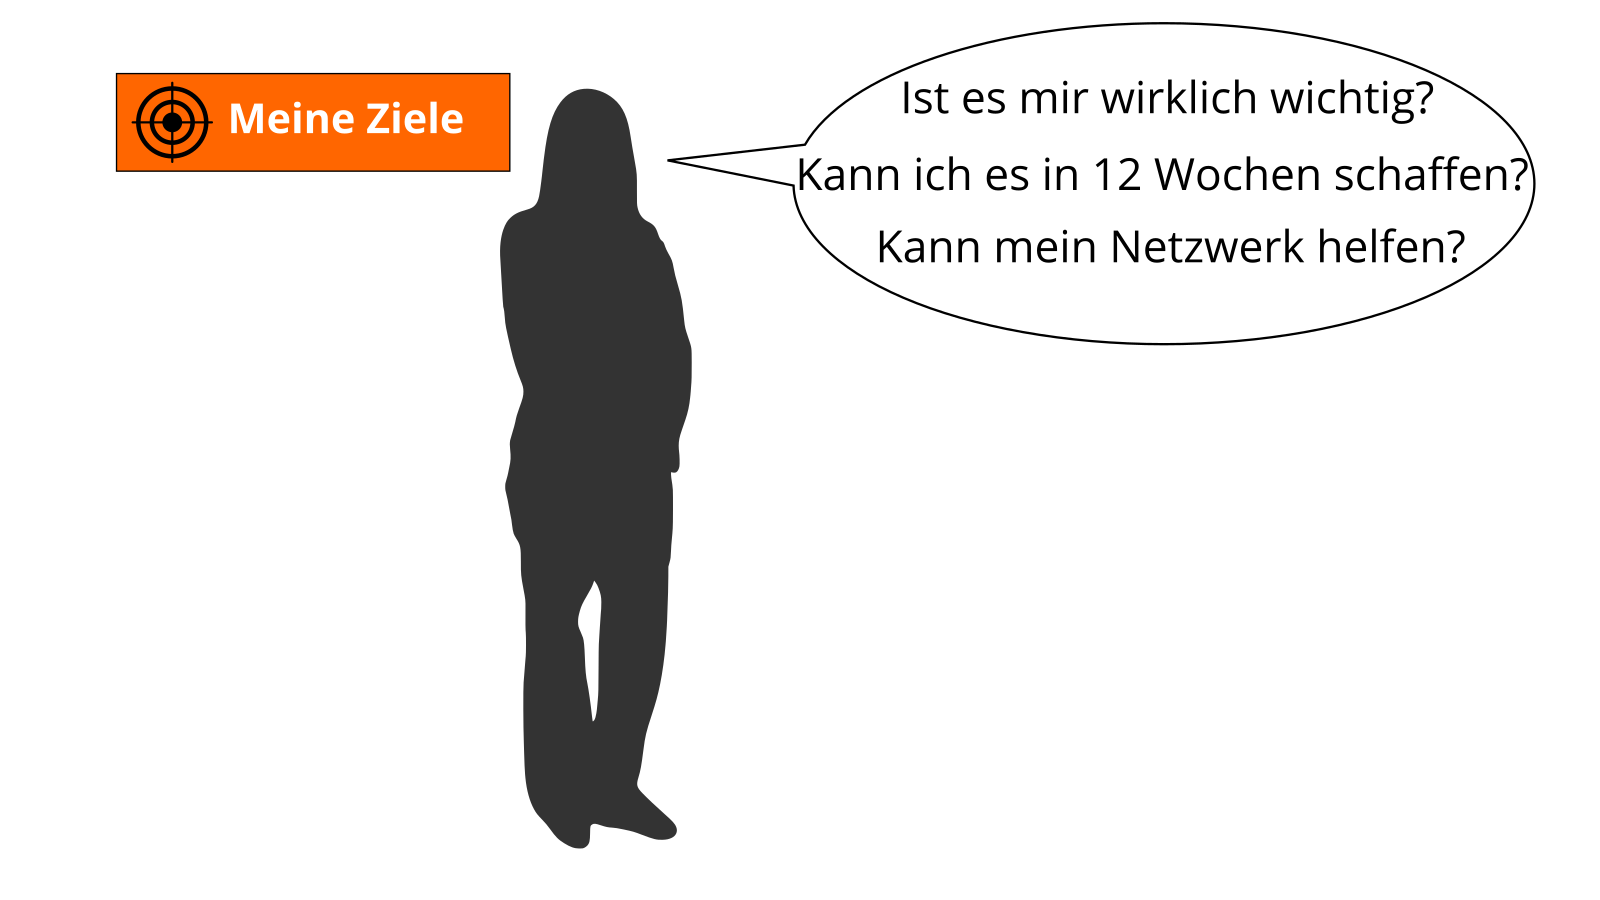
\includegraphics{./tex2pdf.-af94b87e0fdb9aa6/72ba80282397e2812427b590dec7eedfe5393f0e.png}
\caption{Meine Ziele für die nächsten 12 Wochen}
\end{figure}

Wähle ein Ziel für die nächsten 12 Wochen. Verwende die Fragen ``Ist es
mir wirklich, wirklich wichtig?'', ``Kann ich es in 12 Wochen
erreichen?'', und ``Kann mein Netzwerk helfen?'', um zu testen, ob das
Ziel für den Sprint geeignet ist. Wenn du Probleme hast, ein gutes Ziel
zu finden, denke an Ziele zu deine Rollen, Aktivitäten oder Projekten.
Wenn du dazu beitragen möchtes, die Welt zu einem besseren Ort zu
machen, kannst du dir auch ein Ziel aus dem Bereich der
\href{https://www.un.org/sustainabledevelopment/sustainable-development-goals}{17
Ziele für nachhaltige Entwicklung der Vereinten Nationen} wählen.

Verwende die Methode Objective \& Key Results (OKR), um dein Ziel
genauer zu beschreiben. Schreibe unten dein Ziel auf. Definiere 2-4
Schlüsselergebnisse pro Ziel, um dir bei der Fortschrittkontrolle zu
helfen. Du solltest die Schlüsselergebnisse auf einer Skala von 0,0-1,0
messen können. Um sich ehrgeizige Ziele zu setzen, gilt eine
Fertigstellungsrate von 0,7 als Erfolg.

\emph{Ich will (Ziel):} ...

\emph{gemessen an (Schlüsselergebnisse):}

\begin{enumerate}
\def\labelenumi{\arabic{enumi}.}
\tightlist
\item
  \ldots{}
\item
  \ldots{}
\item
  \ldots{}
\item
  \ldots{}
\end{enumerate}

\textbf{Weitere Informationen:}

\begin{itemize}
\tightlist
\item
  Wikipedia Artikel
  \href{https://en.wikipedia.org/wiki/SMART_criteria}{SMART Criteria}
\item
  MIT Sloan Artikel
  \href{https://sloanreview.mit.edu/article/with-goals-fast-beats-smart}{With
  Goals, FAST Beats SMART}
\item
  Ted Talk \href{https://www.youtube.com/watch?v=o08ykAqLOxk}{How We Can
  Make the World a Better Place by 2030}
\item
  Video \href{https://www.youtube.com/watch?v=mJB83EZtAjc}{How Google
  Sets Goals: OKRs} mit Google Ventures Partner Rick Klau
\item
  Buch
  \href{https://www.oreilly.com/business/free/files/introduction-to-okrs.pdf}{Introduction
  To OKRs} von Christina Wodtke
\item
  Buch
  \href{https://felipecastro.com/resource/The-Beginners-Guide-to-OKR.pdf}{The
  Beginner's Guide To OKR} von Felipe Castro
\end{itemize}

\hypertarget{wer-kann-dir-bei-deinem-ziel-helfen-kata-2}{%
\subsubsection{Wer kann dir bei deinem Ziel helfen? (Kata
2)}\label{wer-kann-dir-bei-deinem-ziel-helfen-kata-2}}

In dieser Woche wirst Du über Menschen nachdenken, die Dir bei Deinen
Zielen helfen können (allein arbeiten ist Addition, zusammenarbeiten ist
Multiplikation!).

\textbf{Übung (20 Minuten):}

Die meisten unserer Aufgaben haben andere schon früher erledigt. Die
meisten unserer Fehler, sind schon in der Vergangenheit gemacht worden.
Du kannst Zugang zu diesem Wissen und diesen Erfahrungen erhalten, indem
du mit erfahrenen Menschen in Kontakt trittst. Starke Beziehungen
basieren auf Vertrauen, Teilen und Fürsorge.
\href{https://en.wikipedia.org/wiki/Dale_Carnegie}{Dale Carnegie} sagte:
``Sie können mehr Freunde in zwei Monaten gewinnen, indem Sie sich für
andere Menschen interessieren, als wenn Sie zwei Jahre versuchen, andere
Menschen für sich zu interessieren''. Wie kommst du also mit Menschen in
Kontakt, die mit deinen Zielen in Verbindung stehen und wie kannst du
eine Beziehung mit ihnen aufbauen?

Erstelle eine Liste von mindestens zehn Personen, die mit Deinen Zielen
in Zusammenhang stehen. Wenn du die Leute nicht namentlich kennst,
kannst du auch Rollen oder Beschreibungen auf die Liste setzen (z.B.
``Bester WoW-Spieler in der Stadt'', ``Ein guter Kameramann'',
``Besitzer der Firma XY''). Nutze deine Kontaktlisten oder soziale
Netzwerke, um mehr Personen zu finden:

\begin{enumerate}
\def\labelenumi{\arabic{enumi}.}
\tightlist
\item
  \ldots{}
\item
  \ldots{}
\item
  \ldots{}
\item
  \ldots{}
\item
  \ldots{}
\item
  \ldots{}
\item
  \ldots{}
\item
  \ldots{}
\item
  \ldots{}
\item
  \ldots{}
\end{enumerate}

\textbf{Weitere Informationen:}

\begin{itemize}
\tightlist
\item
  Video \href{https://www.youtube.com/watch?v=6a_KF7TYKVc}{Social
  Networking In Plain English}
\end{itemize}

\hypertarget{teile-etwas-mit-dem-netzwerk-kata-3}{%
\subsubsection{Teile etwas mit dem Netzwerk (Kata
3)}\label{teile-etwas-mit-dem-netzwerk-kata-3}}

In dieser Kata wirst Du Aufmerksamkeit, Wissen, Erfahrungen und
wertvolle Ressourcen mit Deinem Netzwerk teilen, um Vertrauen aufzubauen
und Unterstützung zu erhalten.

\textbf{Übung (40 Minuten):}

Sharing is caring! In der digitalen Welt wird das Teilen oft als
Bereitstellen von Dateien oder digitalen Inhalten gesehen. Aber es geht
auch viel einfacher: Teile deine Aufmerksamkeit mit einer anderen
Person, z.B. indem du ihr folgst, ihre Inhalte ``likest'' oder dir ihre
Website abonnierst. Indem du Aufmerksamkeit teilst, vertiefst du Deine
Beziehungen mit jedem Beitrag, den du machst.

Suche nach einer Online-Präsenz für jede Person in Deiner
Beziehungsliste (z.b. Website, Blog, Profil im sozialen Netzwerk). Suche
nach Möglichkeiten, Aufmerksamkeit zu teilen. Das kann ein
Follow-Button, ein Like-Button, ein Abonnement-Button, eine
5-Sterne-Bewertung, ein Kommentarfeld oder ein Kontaktformular sein.
Mache mindestens fünf Erfahrungen, Aufmerksamkeit zu teilen:

\begin{enumerate}
\def\labelenumi{\arabic{enumi}.}
\tightlist
\item
  \ldots{}
\item
  \ldots{}
\item
  \ldots{}
\item
  \ldots{}
\item
  \ldots{}
\end{enumerate}

\hypertarget{mache-termine-mit-dir-selbst-kata-4}{%
\subsubsection{Mache Termine mit dir selbst (Kata
4)}\label{mache-termine-mit-dir-selbst-kata-4}}

In dieser Woche wirst Du dafür sorgen, dass Du genügend Zeit hast, um
Dich zu vernetzen, zu teilen und Dich um Dein Netzwerk zu kümmern. Du
wirst dies tun, indem Du Termine mit Dir selbst vereinbarst. In dieser
Woche sollte Dein Ziele stabil sein und Du solltest eine klare
Vorstellung haben, welche Leute im Netzwerk Dir helfen könnten, Deine
Dinge zu erledigen. Nehmt Euch diese Woche einen kurzen ``Boxenstopp'',
um zu reflektieren, ob alles gut für Dich und den Circle funktioniert.
In den nächsten vier Wochen wirst Du Dich darauf konzentrieren, an der
ersten Iteration Deiner Key Results zu arbeiten.

\textbf{Übung (15 Minuten):}

Nimmst du dir ausreichend Zeit für deine persönliche Entwicklung und für
die Arbeit an deinen Zielen? Viele Menschen sind mit ihren täglichen
Aufgaben beschäftigt und kümmern sich nicht genug um Ihre Entwicklung
und Ihr Wohlbefinden. Ein guter Ansatz ist es, einen Termin mit sich
selbst zu vereinbaren und sich diese Zeit im Kalender zu reservieren.

Überprüfe deinen Kalender und suche nach möglichen Terminen mit Dir
selbst. Eine Stunde oder sogar 30 Minuten pro Woche ist ein guter
Ausgangspunkt. Trage dir einen Termin mit dir selbst in den Kalender
ein. Mache ihn nach Möglichkeit zu einem wiederkehrenden Termin, damit
diese Zeit für Dich zur Gewohnheit wird. Finde mindestens fünf Termine:

\begin{enumerate}
\def\labelenumi{\arabic{enumi}.}
\tightlist
\item
  \ldots{}
\item
  \ldots{}
\item
  \ldots{}
\item
  \ldots{}
\item
  \ldots{}
\end{enumerate}

\hypertarget{egosurfe-dich-kata-5}{%
\subsubsection{Egosurfe dich! (Kata 5)}\label{egosurfe-dich-kata-5}}

In dieser Kata wirst Du Dich selber im Intranet oder Internet suchen.

\textbf{Übung (10 Minuten):}

Was sehen Menschen, die Dich im Netz suchen? Bekommen sie eine
Vorstellung davon, wer du bist und wie sie Dir bei deinen Zielen helfen
können? Du kannst diese Situation simulieren, indem du Dich selbst
googelst (oft als egosurfing, egosearch oder vanity search bezeichnet).


\includegraphics{./tex2pdf.-af94b87e0fdb9aa6/da4901626a83ec7029c76ad718e7f83d3f629d0f.png}

Öffne eine Suchmaschine im Netz und gebe Deinen Namen ein. Öffne
mindestens die ersten zehn Suchergebnisse und prüfe, ob deine
Persönlichkeit und die Fakten über Dich auf dem neuesten Stand sind.
Identifiziere mögliche Verbesserungsmaßnahmen:

\begin{enumerate}
\def\labelenumi{\arabic{enumi}.}
\tightlist
\item
  \ldots{}
\item
  \ldots{}
\item
  \ldots{}
\item
  \ldots{}
\item
  \ldots{}
\item
  \ldots{}
\item
  \ldots{}
\item
  \ldots{}
\item
  \ldots{}
\item
  \ldots{}
\end{enumerate}

Denke darüber nach, was dein zentrales Online-Profil sein könnte (z.B.
LinkedIn-Profil, about.me-Profil oder Profil im Enterprise Social
Network). Dieses Profil wird im Folgenden dein ``digitaler Zwilling''
genannt. Der digitale Zwilling repräsentiert Dich im Netz:

\emph{Mein zentrales Online-Profil (Digital Twin) ist \ldots{}}

\textbf{Weitere Informationen:}

\begin{itemize}
\tightlist
\item
  Wikipedia Artikel
  \href{https://en.wikipedia.org/wiki/Egosurfing}{Egosurfing}
\item
  Artikel
  \href{https://snurb.info/files/aoir2008/Google\%20Yourself!\%20Measuring\%20the\%20performance\%20of\%20personalized\%20information\%20resources\%20\%28AoIR\%202008\%29.pdf}{Google
  Yourself! Measuring the performance of personalized information
  resources} von Thomas Nicolai und Lars Kirchhoff.
\end{itemize}

\hypertarget{beschreibe-dich-in-25-tags-kata-6}{%
\subsubsection{Beschreibe dich in 25 Tags (Kata
6)}\label{beschreibe-dich-in-25-tags-kata-6}}

In dieser Kata wirst Du Fakten und persönliche Informationen sammeln,
die für Dein Netzwerk relevant sein könnten und Dir helfen, Dich zu
vernetzen.

\textbf{Übung (25 Minuten):}

Welche interessanten Fakten über Dich können dir helfen, Dich mit
anderen Menschen zu vernetzen? Wenn du Dich für ein Studium an der Fuqua
Business School bewerben willst, musst du einen Aufsatz mit einer Liste
von 25 zufälligen Dingen über Dich selbst schreiben, damit das
Bewerbungsteam Dich besser kennenlernt. Wenn du die Fakten über dich
selbst aufschreibst, sammele Informationen, die dir helfen könnten, neue
Beziehungen zu knüpfen, die auf ähnlichen Interessen und Hintergründen
basieren (z.B. ``Wir haben vor 20 Jahren am gleichen Ort studiert!'').
Fakten über Dich selbst sind beispielsweise:

\begin{itemize}
\tightlist
\item
  Lebenserfahrungen
\item
  Deine Vorlieben/Abneigungen
\item
  Wo du geboren wurdest/lebst
\item
  Familie, Kinder, Eltern
\item
  Schulen, Universitäten
\item
  Arbeitsplätze in der Vergangenheit
\item
  Berufliche Herausforderungen
\item
  Urlaube
\item
  Hobbys
\item
  Leistungen
\item
  Lustige Fakten
\item
  Alles, was hilft zu verstehen, was Dich ausmacht und wer du bist
\end{itemize}

Erstelle eine Liste von zehn Fakten über Dich selbst. Dann lies die
\href{https://stratusadmissionscounseling.com/duke-fuqua-25-random-things-dos-donts}{``Fuqua
25 random things do's and dont's''} und erweitere deine Liste auf 25
Fakten:

\begin{enumerate}
\def\labelenumi{\arabic{enumi}.}
\tightlist
\item
  \ldots{}
\item
  \ldots{}
\item
  \ldots{}
\item
  \ldots{}
\item
  \ldots{}
\item
  \ldots{}
\item
  \ldots{}
\item
  \ldots{}
\item
  \ldots{}
\item
  \ldots{}
\item
  \ldots{}
\item
  \ldots{}
\item
  \ldots{}
\item
  \ldots{}
\item
  \ldots{}
\item
  \ldots{}
\item
  \ldots{}
\item
  \ldots{}
\item
  \ldots{}
\item
  \ldots{}
\item
  \ldots{}
\item
  \ldots{}
\item
  \ldots{}
\item
  \ldots{}
\item
  \ldots{}
\end{enumerate}

\textbf{Weitere Informationen:}

\begin{itemize}
\tightlist
\item
  YouTube-Suche
  \href{https://www.youtube.com/results?search_query=random+facts+about+me}{``random
  facts about me''}
\end{itemize}

\hypertarget{aktualisiere-deinen-digitalen-zwilling-kata-7}{%
\subsubsection{Aktualisiere deinen digitalen Zwilling (Kata
7)}\label{aktualisiere-deinen-digitalen-zwilling-kata-7}}

In dieser Kata wirst Du, wenn Deine digitalen Zwillinge wie Website,
Blog oder Profil nicht mit Deinen Erkenntnissen aus der letzten Woche
übereinstimmen, diese aktualisieren.

\textbf{Übung (20 Minuten):}

Stellt dein digitaler Zwilling Dich so dar, wie du es möchtest? Viele
Menschen melden sich in einem sozialen Netzwerk an und aktualisieren Ihr
Profil nie mehr. Du solltest dein Profil auf dem neuesten Stand halten
und regelmäßig überprüfen (z.B. wiederkehrende Aufgabe alle drei
Monate). Die Fakten über Dich, aktuelle Projekte und aktuelle Interessen
sollten auf dem Profil sichtbar sein.

Überprüfe im Online-Profil, ob du ein ansprechendes Bild, eine kurze
Beschreibung und einen Slogan hast. Liste Verbesserungsideen auf, die du
umsetzen möchtest:

\begin{enumerate}
\def\labelenumi{\arabic{enumi}.}
\tightlist
\item
  \ldots{}
\item
  \ldots{}
\item
  \ldots{}
\item
  \ldots{}
\item
  \ldots{}
\item
  \ldots{}
\item
  \ldots{}
\item
  \ldots{}
\item
  \ldots{}
\item
  \ldots{}
\end{enumerate}

\hypertarget{poste-deine-top-10-truxfcffel-kata-8}{%
\subsubsection{Poste deine Top 10 Trüffel (Kata
8)}\label{poste-deine-top-10-truxfcffel-kata-8}}

In dieser Kata wirst Du zu Deinen Top 10 Wissenswerte reflektieren, die
Du in Deinem Netzwerk teilen kannst.

\textbf{Übung (30 Minuten):}

Was sind die wichtigsten Ressourcen im Zusammenhang mit deinen Zielen,
die du teilen kannst? Eine Ressource kann ein Buch, ein Video, ein Link,
ein Dokument, eine Checkliste, eine Präsentation etc. sein. Wenn deine
Ressourcen einfach per Link teilbar sind, kannst du sie unkompliziert im
Netzwerk teilen.

Wähle eines Deiner Ziele und schreibe mindestens zehn Ressourcen auf,
die dafür nützlich oder interessant sind:

\begin{enumerate}
\def\labelenumi{\arabic{enumi}.}
\tightlist
\item
  \ldots{}
\item
  \ldots{}
\item
  \ldots{}
\item
  \ldots{}
\item
  \ldots{}
\item
  \ldots{}
\item
  \ldots{}
\item
  \ldots{}
\item
  \ldots{}
\item
  \ldots{}
\end{enumerate}

\hypertarget{welche-kanuxe4le-willst-du-nutzen-kata-9}{%
\subsubsection{Welche Kanäle willst du nutzen? (Kata
9)}\label{welche-kanuxe4le-willst-du-nutzen-kata-9}}

\ldots{} Blog, Vlog, Podcast etc. \ldots{}

\textbf{Übung (Minuten):}

\ldots{}

\hypertarget{welche-communities-kuxf6nnen-dir-helfen-kata-10}{%
\subsubsection{Welche Communities können dir helfen? (Kata
10)}\label{welche-communities-kuxf6nnen-dir-helfen-kata-10}}

In dieser Kata nach Communities oder Gruppen suchen, die Dir helfen
können, Deine Ziele zu erreichen.

\textbf{Übung (15 Minuten):}

Ein ``Tribe'' ist
\href{https://www.ted.com/talks/seth_godin_on_the_tribes_we_lead}{laut
Seth Godin} eine Gruppe von Menschen, die mit einem Anführer und einer
Idee verbunden ist. Anstelle von Tribe wird oft auch der Begriff
``Community'' oder ``Community of Practice'' (Praxisgemeinschaft)
verwendet. Eine Gruppe braucht zwei Dinge zur Interaktion: ein
gemeinsames Interesse und eine Möglichkeit zu kommunizieren. Communities
brauchen Führung. Manchmal führt eine Person, manchmal mehrere. Welches
sind die Communities, die mit deinen Zielen in Zusammenhang stehen?

Suche nach Communities, die mit deinen Zielen in Zusammenhang stehen,
und finde mindestens zehn (verwende z.B.
\href{https://www.linkedin.com/groups}{LinkedIn-Gruppen},
\href{https://www.facebook.com/groups}{Facebook Groups},
\href{https://www.xing.com/communities}{XING Groups} ,
\href{https://www.meetup.com}{Meetup.com},
\href{https://www.reddit.com/reddits}{Reddit.com}):

\begin{enumerate}
\def\labelenumi{\arabic{enumi}.}
\tightlist
\item
  \ldots{}
\item
  \ldots{}
\item
  \ldots{}
\item
  \ldots{}
\item
  \ldots{}
\item
  \ldots{}
\item
  \ldots{}
\item
  \ldots{}
\item
  \ldots{}
\item
  \ldots{}
\end{enumerate}

\hypertarget{schreibe-einen-brief-an-dein-zukuxfcnftiges-ich-kata-11}{%
\subsubsection{Schreibe einen Brief an dein zukünftiges Ich (Kata
11)}\label{schreibe-einen-brief-an-dein-zukuxfcnftiges-ich-kata-11}}

In dieser Kata wirst Du Dir Dich selbst in der Zukunft vorstellen, indem
Du einen Brief an Dein zukünftiges ich schreibst. Und Du hilfst Deinem
Netzwerk, Dich zu unterstützen, indem Du Deine Vision und Deine Ziele
auf Deinen Online-Profilen sichtbar machst.

\textbf{Übung (35 Minuten):}

Der Brief an dein zukünftiges Ich ist eine klassische Methode zur
Selbstmotivation. Du reflektierst deine aktuelle Situation und gibst
Deinem zukünftigen Ich einen Rat. Du schreibst den Brief, adressierst
ihn an Dich selbst und öffnest ihn in der Zukunft. Mit dem Brief im
Hinterkopf erhöht sich die Wahrscheinlichkeit, dass deine Wünsche eine
\href{https://en.wikipedia.org/wiki/Self-fulfilling_prophecy}{sich
selbst erfüllende Prophezeiung} werden.

Schreibe einen Brief an dein zukünftiges Ich. Sprich darüber, wer du
jetzt bist (z.B. Zusammenfassung, Ängste, Werte, Überzeugungen,
Fähigkeiten, Fertigkeiten, Ziele, Hoffnungen). Dann erläutere Deinem
zukünftigen Ich die Dinge, die du stoppen/weitermachen/anfangen
möchtest. Gib ihm Ratschläge und stelle ihm Fragen. Verschließe den
Brief und verwahre ihn an einem sicheren Ort oder nutze Online-Dienste
wie \href{https://futureme.org}{futureme.org} um ihn automatisch an Dein
zukünftiges Selbst zu senden:


\includegraphics{./tex2pdf.-af94b87e0fdb9aa6/15a0f9300a5b0066a418f759ebc52be34fb130a8.png}

\textbf{Weitere Informationen:}

\begin{itemize}
\tightlist
\item
  Video \href{https://www.youtube.com/watch?v=XwN0tJlXF-0}{A Letter To
  My Future Self}
\item
  Artikel
  \href{https://www.wikihow.com/Write-a-Letter-to-Your-Future-Self}{How
  to Write a Letter to Your Future Self}
\end{itemize}

\hypertarget{okr-lernpfad}{%
\subsection{OKR Lernpfad}\label{okr-lernpfad}}

Sich selbst ambitionierte Ziele (Objectives) zu stecken und greifbare
Ergebnisse (Key Results) zu definieren, kann sehr motivierend sein.
Viele Menschen haben eine lange Man-Müsste-Mal-Liste, gehen dieses Ziele
aber nicht richtig an. Je länger die Liste, desto größer die Hürde etwas
anzupacken. Google verwendet daher die einfache Methode Objectives \&
Key Results (OKR) bei der die Ziele der nächsten drei Monate
\href{https://rework.withgoogle.com/guides/set-goals-with-okrs/steps/introduction/}{nach
folgenden Kriterien} definiert werden:

\begin{itemize}
\tightlist
\item
  Objectives sind anspruchsvoll und können sich etwas unbequem anfühlen.
\item
  Key Results sind auf einer Skala von 0 - 1,0 messbar (oder 0-100\%).
\item
  OKRs sind transparent, so dass jeder sehen kann, woran andere
  arbeiten.
\item
  Der optimale Grad der Zielerreichung ist 60-70\%. Wenn du deine Ziele
  immer zu 100\% erreichst, sind deine OKRs nicht ambitioniert genug und
  du solltest dir höhere Ziele stecken.
\item
  Ein niedriger Grad der Zielerreichung sollte als Lernchance für die
  nächsten OKRs angesehen werden.
\item
  In Unternehmen dienen OKRs NICHT(!) zur Leistungsbeurteilung.
\item
  OKRs sind keine geteilte Aufgabenliste.
\end{itemize}

Mit den folgenden Katas, kannst du OKRs für das Stecken eigener Ziele in
einem Sprint erlernen. Dabei ist es egal, ob du in einer Organisation
oder einem Unternehmen bist, das bereits OKR einsetzt oder ob du OKRs
einfach für dich selber nutzen magst.

\hypertarget{top-10-quellen-zu-okrs-kata}{%
\subsubsection{Top 10 Quellen zu OKRs
(Kata)}\label{top-10-quellen-zu-okrs-kata}}

\textbf{Lerne etwas über die Geschichte und die Grundlagen von
Objectives \& Key Results (OKRs).}

\emph{\textbf{Dauer:} 60 Minuten}

Die Geschicht von OKRs reicht einige Jahrzehnte zurück. 1975 nahm John
Doerr bei Intel an einer Schulung teil, in der Andy Grove die Theorie
von OKRs erklärte (Buch-Tipp: \href{https://amzn.to/2O9sA4u}{High Output
Management}). 1999 arbeitete John Doerr für das Venture Capital
Unternehmen Kleiner Perkins Caufield \& Byers, das gerade in das Startup
Google investiert hatte. Darüber gelangte die Methode OKR zu Google. im
Vorwort des Buchs \href{https://amzn.to/2XVI1Bv}{Measure What Matters:
OKRs: The Simple Idea that Drives 10x Growth} von Doerr beschreibt
Google-Gründer Larry Page die Wirkung von OKRs so:

\begin{quote}
OKRs have helped lead us to 10x growth, many times over. They've helped
make our crazily bold mission of `organizing the world's information'
perhaps even achievable. They've kept me and the rest of the company on
time and on track when it mattered the most.
\end{quote}

Im Folgenden habe ich einige Quellen zusammengestellt, mit denen du dich
mit der Methode vertraut machen kannst. Suche dir aus folgender Liste
Materialen aus und lerne die Grundlagen von OKRs kennen:

\begin{enumerate}
\def\labelenumi{\arabic{enumi}.}
\tightlist
\item
  \textbf{\href{https://rework.withgoogle.com/guides/set-goals-with-okrs/steps/introduction}{Set
  Goals with OKRs}} (en) - wenn du nur eine Quelle wählst, nimm diese!
  Google beschreibt auf ca. 10 Seiten wie sie OKRs zur agilen
  Zielplanung verstehen und verwenden.
\item
  \textbf{\href{https://en.wikipedia.org/wiki/OKR}{OKR}} (en) -
  englischsprachige Wikipedia-Seite zu OKRs mit vielen Weblinks und
  Quellen. Über die Sprachumschaltung in der linken Seitenleiste sind
  weitere Informationen in anderen Wikipedia-Sprachversionen zugänglich.
\item
  \textbf{\href{https://www.youtube.com/watch?v=mJB83EZtAjc}{How Google
  sets goals: OKRs}} (en) - Videoaufzeichung (1 Stunde 22 Minuten) eines
  Startup Lab Workshops mit Rick Klau von Google Ventures, in dem Rick
  auch originale Folien von John Doerr zeigt.
\item
  \textbf{\href{https://www.oreilly.com/business/free/files/introduction-to-okrs.pdf}{Introduction
  to OKRs}} (en)- 37-seitige Einführung in OKR von Christina Wodtke
  ({[}@cwodtke{]}(https://twitter.com/cwodtke)) mit der Geschichte und
  konkreten Tipps zum Start mit OKRs.
\item
  \textbf{\href{https://felipecastro.com/resource/The-Beginners-Guide-to-OKR.pdf}{The
  Beginner's Guide to OKR}} - 50-seitige Einführung in OKRs von Felipe
  Castro ({[}@meetfelipe{]}(https://twitter.com/meetfelipe)) mit vielen
  Beispielen und konkreten Handlungshilfen.
\item
  \textbf{\href{http://okrbook.com}{Objectives and Key Results: The
  Book}} (en) - 31-seitiges eBook von Alexander Maasik
  ({[}@AMaasik{]}(https://twitter.com/AMaasik)) mit Grundlagen zu OKRs
  und Beispielen aus der Software \href{https://weekdone.com}{weekdone}.
\item
  \textbf{\href{https://www.okrs.com/2016/12/bens-white-paper}{Objectives
  and Key Results}} (en) - White Paper von Ben Lamorte () Betreiber der
  Webseite \href{https://okrs.com}{okrs.com}.
\item
  \textbf{\href{https://www.therebegiants.com/the-official-okr-podcast}{Giant
  Talk Podcast}} (en) - Podcast zur OKRs von There Be Giants, einer
  OKR-Beratung aus Großbritannien.
\item
  \textbf{\href{https://www.workpath.com/wp-content/uploads/2018/10/okr-community-report2017.pdf}{OKR
  Community Report 2017}} (en) - Umfrage des Workpath Institute mit über
  300 Teilnehmenden und Fallbeispielen von HolidayCheck, MyMuesli und
  Flixbus.
\item
  \textbf{\href{https://www.workpath.com/okr-plus}{OKRs und digitale
  Organisationen}} (de) - Einführung in OKRs von
  \href{https://workpath.com}{workpath}, einem OKR-Software-Anbieter aus
  München.
\end{enumerate}

\hypertarget{richte-deine-okr-umgebung-ein-kata}{%
\subsubsection{Richte deine OKR-Umgebung ein
(Kata)}\label{richte-deine-okr-umgebung-ein-kata}}

\textbf{Plane Zeit und Raum für deinen OKR-Prozess ein.}

\emph{\textbf{Dauer:} 30 Minuten}

Für deine persönliche OKR-Umgebung braucht es nicht viel. Du musst dir
wöchentlich Zeit für das Weekly Check-in im Kalender einplanen (z.B.
Montag Morgen, 30 Minuten). Außerdem benötigst du eine Stelle, an der du
deine OKRs dokumentierst. Diese Stelle kann analog (z.B. Papier,
Whiteboard) oder digital (z.B. OneNote, Wiki) sein. Du musst
entscheiden, ob du deine OKRs gleich beim ersten Mal öffentlich machst
oder nicht. Bedenke: je kleiner der Kreis der Personen, die deine Ziele
kennen, desto weniger können dir bei der Erreichung der Ziele helfen.

Lege jetzt deine OKR-Umgebung fest:

\begin{itemize}
\tightlist
\item
  \textbf{OKR Weekly Check-in (Wochentag, Uhrzeit):} \ldots{}
\item
  \textbf{OKR Dokumentation:} \ldots{}
\end{itemize}

\hypertarget{definiere-okrs-fuxfcr-deinen-sprint-kata}{%
\subsubsection{Definiere OKRs für deinen Sprint
(Kata)}\label{definiere-okrs-fuxfcr-deinen-sprint-kata}}

\textbf{Schreibe dein Ziel (Objective) und die Schlüsselergebnisse (Key
Results) für diesen Sprint im OKR-Format auf.}

\emph{\textbf{Dauer:} 30 Minuten}

In der letzten Kata hast du (hoffentlich) einiges über die Formulierung
von OKRs gelernt. Jetzt kannst du das auf die Zielplanung für den
laufenden Sprint anwenden. Verwende dazu die OKR-Formel von John Doer,
um dein Ziel zu formulieren:

\emph{Ich will (Objective): \ldots\ldots\ldots. gemessen an
\ldots\ldots\ldots. (Key Results):}

Überprüfe dein \textbf{Objective} anhand folgender Kriterien (Quelle:
\href{https://rework.withgoogle.com/guides/set-goals-with-okrs/steps/set-objectives-and-develop-key-results/}{Google}):

\begin{itemize}
\tightlist
\item
  Das Objective ist anspruchsvoll und fühlt sich ein bisschen unbequem
  an.
\item
  Das Objective verwendet Formulierungen, die neue Aktivitäten anstoßen
  (nicht: beibehalten, weitermachen).
\item
  Das Objective verwendet Formulierungen, die einen Endzustand
  beschreiben (z.B. ``climb the mountain'', ``ship feature Y'').
\item
  Das Objective verwendet greifbare und unmissverständliche Begriffe.
  Für einen Aussenstehenden sollte klar sein, ob ein Ziel erreicht wurde
  oder nicht.
\end{itemize}

Überprüfe deine \textbf{Key Results} anhand folgender Kriterien:

\begin{itemize}
\tightlist
\item
  Pro Objective sind nicht mehr als drei Key Results definiert.
\item
  Die Key Results drücken messbare Meilensteine aus, die einen bei
  Erreichung dem Ziel näher bringen.
\item
  Die Key Results sind messbar und können auf einer Skala von 0,0 - 1,0
  (oder 0 - 100\%) gemessen werden.
\item
  Die Key Results drücken Ergebnisse, nicht Tätigkeiten aus. Die
  Formulierung eines Key Results sollte keine Wörter wie ``beraten'',
  ``helfen'', ``analysieren'' oder ``teilnehmen'' enthalten.
\item
  Messbare Meilensteine sollten den Nachweis der Fertigstellung
  beinhalten. Und diese Nachweise sollten sichtbar, glaubwürdig und
  leicht nachvollziehbar sein.
\end{itemize}

\hypertarget{finalisiere-deine-okrs-fuxfcr-den-sprint-kata}{%
\subsubsection{Finalisiere deine OKRs für den Sprint
(Kata)}\label{finalisiere-deine-okrs-fuxfcr-den-sprint-kata}}

\textbf{Überprüfe deine OKRs für den Sprint und lege dich fest.}

\emph{\textbf{Dauer:} 30 Minuten}

Du hattest jetzt einige Nächte, um deine OKRs nochmal zu überdenken.
Fühlst du dich wohl und motiviert damit? Fühlen sich die Objectives
anspruchsvoll an? Siehst du eine realistische Chance die Key Results zu
60-70\% erreichen zu können. Überdenke deine OKRs nochmal und lege dich
für diesen Sprint fest. Dokumentiere die OKRs dann in deiner
OKR-Umgebung.

\hypertarget{fuxfchre-dein-weekly-check-in-durch-kata}{%
\subsubsection{Führe dein Weekly Check-In durch
(Kata)}\label{fuxfchre-dein-weekly-check-in-durch-kata}}

\textbf{Starte mit einem kurzen OKR Weekly Check-In in jede Woche}

\emph{\textbf{Dauer:} 30 Minuten}

Mit dem OKR Weekly Check-in kannst du dir deine Ziele und den aktuellen
Stand wöchentlich vor Augen führen. Das hilft dir, nicht den Fokus zu
verlieren und Hindernisse frühzeitig zu erkennen und aus dem Weg zu
räumen.

Den Zeitpunkt deines Check-in hast du ja bereits festgelegt und als
Regeltermin im Kalender stehen. Verwende folgende Fragen für das OKR
Weekly Check-in:

\begin{itemize}
\tightlist
\item
  \textbf{Fortschritt:} Was hat sich bei den Key Results seit dem
  letzten Weekly geändert?
\item
  \textbf{Vertrauen:} Wie sicher bin ich mir, die Key Results zu
  erreichen?
\item
  \textbf{Barrieren:} Was behindert mich in meinem Fortschritt?
\item
  \textbf{Nächste Schritte:} Was kann ich tun, um den Fortschritt zu
  verbessern?
\end{itemize}

Verwende die kommenden vier Wochen, um das Check-in zu einer
wöchentlichen Routine zu machen. In jeder Woche lernst du in kleinen
Lernhäppchen von 15 Minuten zusätzliche Themen rund um OKRs kennen.

\hypertarget{tools-fuxfcr-okrs-kata}{%
\subsubsection{Tools für OKRs (Kata)}\label{tools-fuxfcr-okrs-kata}}

\textbf{Lerne einige Tools für OKRs kennen.}

\emph{\textbf{Dauer:} 15 Minuten}

David Allen beschreibt Getting Things Done (GTD) oft als
``tool-agnostic''. D.h. man kann GTD unabhängig von spezieller Software
oder Apps praktizieren. Ähnlich ist es mit OKRs, Papier und Bleistift
reichen, trotzdem verwenen viele Praktiker digitale Werkzeuge dafür.
Beschäftige dich in dieser Woche mit Beispielen von OKR-Tools und
entscheide, ob du davon welche nutzen möchtest:

\begin{itemize}
\tightlist
\item
  \textbf{Textverareitung}, z.B. Microsoft Word, Google Doc
\item
  \textbf{Tabellenkalkulation}, z.B. Microsoft Excel, Google Sheets
\item
  \textbf{Notizanwendungen}, z.B. Microsoft OneNote, Evernote
\item
  \textbf{To-Do-Listen-Tools}, z.B. Trello, Microsoft To-Do, Microsoft
  Planner, Jira
\item
  \textbf{Wikis}, z.B. Mediawiki, Confluence, TiddlyWiki, Etherpad
\item
  \textbf{Enterprise OKR-Tools}, z.B. 7Geese, WeekDone, Workpath
\end{itemize}

\hypertarget{scoring-vs.-measuring-key-results-kata}{%
\subsubsection{Scoring vs.~Measuring Key Results
(Kata)}\label{scoring-vs.-measuring-key-results-kata}}

\textbf{Verstehe den Unterschied zwischen ``Scoring'' und ``Measuring''
und entscheide dich für deinen Weg.}

\emph{\textbf{Dauer:} 15 Minuten}

Google empfiehlt für OKRs die Key Results immer auf einer Skala von 0 -
1,0 messen zu können. In seinem
\href{https://felipecastro.com/resource/The-Beginners-Guide-to-OKR.pdf}{Beginners
Guide to OKR} beschreibt Felipe Castro unter der Überschrift ``Forget
Scoring'' einige Nachteile dieses Ansatzes:

\begin{itemize}
\tightlist
\item
  Die Bewertung auf der Skala von 0 - 1,0 ist sehr subjektiv
\item
  Wenn man im Vorfeld pro Key Result festlegen will, was 0,3, 0,7 etc.
  bedeutet, steigt die Komplexität des Prozesses
\end{itemize}

Daher empfiehlt Felipe die Key Results nicht auf der Skala von 0 - 1,0
zu ``scoren'', sondern Wert-basierte Key Results zu verwenden und die
einfach zu messen. Seiner Meinung nach vereinfacht das den Prozess der
Definition von OKRs für einen selber und auch für Teams.

Schaue dir deine Key Results an und überlege, ob sich der Prozess für
dich durch einfaches Messen statt der Bewertung auf der Skala von 0 -
1,0 vereinfachen würde. Entscheide dich für eine Vorgehensweise und
passe deine Key Results ggf. an.

\hypertarget{stretch-goals-and-moonshots-kata}{%
\subsubsection{Stretch Goals and Moonshots
(Kata)}\label{stretch-goals-and-moonshots-kata}}

\textbf{Lerne die Bedeutung von ``Strech Goals'' für das Stecken
anspruchsvoller Ziele kennen.}

\emph{\textbf{Dauer:} 15 Minuten}

Mit Strech Goals oder Moonshot OKRs (abgeleitet von Kennedy's Moonshot
Goal 1962) werden Ziele bezeichnet, die unmöglich zu erreichen scheinen.
Man kann sich z.B. mal nicht fragen ``Wie werde ich um 10\%
besser/schneller?'', sondern ``Wie werde ich um den Faktor 10
besser/schneller''. Dadurch wird man gezwungen, die eigene Komfortzone
zu verlassen und über andere Praktiken, Fähigkeiten und anders Know-how
nachzudenken.

Schaue dir deine Objectives an und überlege, aus welchen du Moonshot
OKRs machen könntest und welche Konsequenzen das für dich hätte. Wenn du
Moonshot OKRs ausprobieren möchtest, entscheide, ob du die OKRs noch für
diesen oder einen folgenden Sprint anpassen möchtest.

\hypertarget{what-is-your-confidence-level-kata}{%
\subsubsection{What is your Confidence Level?
(Kata)}\label{what-is-your-confidence-level-kata}}

\textbf{Wie sicher bist du dir, dass du deine OKRs erreichen wirst?}

\emph{\textbf{Dauer:} 15 Minuten}

Nach Henrik-Jan van der Pol von perdoo zeigt der
\href{https://www.perdoo.com/blog/okr-confidence-levels/}{OKR Confidence
Level} als Indikator an, wie sehr du daran glaubst, dass das OKR (noch)
erreichbar ist. Henrik-Jan schlägt die drei Stufen ``on-track'',
``off-track'' und ``at-risk'' vor. Die Schätzung eines OKD Confidence
Levels wird auch von Christina Wodtke im Buch
\href{https://www.oreilly.com/business/free/files/introduction-to-okrs.pdf}{Introduction
to OKRs} vor. Sie empfiehlt eine Skala von 1-10, wobei eine 1 heisst
``Es müsste ein Wunder geschehen'' und eine 10 ``Yeah, das schaffe
ich''.

Schaue dir die beiden Quellen an und entscheide, ob du für deine OKRs
auch Confidence Level schätzen möchtest. Wenn ja, überlege, wo und wann
du diese in deiner Dokumentation pflegst.

\hypertarget{individual-vs.-teamorganizational-okrs-kata}{%
\subsubsection{Individual vs.~Team/Organizational OKRs
(Kata)}\label{individual-vs.-teamorganizational-okrs-kata}}

\textbf{Lerne das Zusammenspiel von OKRs auf den Ebenen Individuum, Team
und Organisation kennen.}

\emph{\textbf{Dauer:} 30 Minuten}

Wie im Video \href{https://youtu.be/mJB83EZtAjc?t=1061}{How Google sets
goals: OKRs} von Rick Klau gut beschrieben, werden OKRs nicht nur auf
individueller Ebene, sondern auch auf Ebene von Teams, Abteilungen und
der ganzen Organisation definiert. Im Gegensatz zu anderen
Zielvereinbarungssystemen wie beispielsweise
\href{https://de.wikipedia.org/wiki/Management_by_Objectives}{Management
by Objectives} (MbO) ist das aber kein reiner Top-Down-Prozess, sondern
erfolgt sowohl Top-Down (Empfehlung John Doerr: 40\%), als auch
Bottom-Up (Empfehlung John Doerr: 60\%).

Überlege, ob du neben deinen persönlichen OKRs die Methode auch in
deinem Umfeld, wie beispielsweise deinem Team oder deiner Abteilung
einsetzen kannst. Überlege dir mindestens eine Maßnahme, um zu testen,
ob dein Umfeld offen für OKRs ist und wie man das dort umsetzen könnte.

\hypertarget{okr-review-kata}{%
\subsubsection{OKR Review (Kata)}\label{okr-review-kata}}

\textbf{War dein OKR Zyklus erfolgreich und welche Themen ergeben sich
für den nächsen?}

\emph{\textbf{Dauer:} 60 Minuten}

In Scrum dient der
\href{https://www.scrumguides.org/scrum-guide.html\#events-review}{Sprint
Review} dazu, am Ende des Sprints die Ergebnisse (Inkremente) zu prüfen
(Inspect) und bei Bedarf für den nächsten Sprint anzupassen (Adapt). In
Scrum ist das Review von der
\href{https://www.scrumguides.org/scrum-guide.html\#events-retro}{Sprint
Retrospektive} zu unterscheiden, bei der es um die Interaktion im Team
und nicht die Ergebnisse geht.

Franziska Schneider von Workpath
\href{https://www.workpath.com/magazine/wie-sie-einen-effektiven-okr-zyklus-gestalten/}{schlägt
in einem Blog vor}, zum Abschluss eines OKR Zyklus auch ein Review zu
machen und sich dabei folgende Fragen zu stellen:

\begin{itemize}
\tightlist
\item
  War ich mit meinen OKRs erfolgreich?
\item
  Welche Themen ergeben sich für den nächsten OKR Zyklus?
\item
  Wo kann/sollte ich die Ergebnisse des Reviews präsentieren?
\end{itemize}

Führe jetzt ein OKR Review für den aktuellen Sprint durch und
dokumentiere die Ergebnisse.

\hypertarget{gtd-lernpfad}{%
\subsection{GTD Lernpfad}\label{gtd-lernpfad}}

Sich selbst und seine Arbeitsweise zu organisieren und zu optimieren
kann sehr motivierend sein. Viele Menschen stehen heute vor dem Problem,
im Hamsterrad der Tages- und Routinetätigkeiten zu versinken und keine
Zeit für wertschöpfende Dinge zu haben, geschweigen denn sich Gedanken
darüber zu machen, wohin sie sich mittel- bis langfristig entwickeln
wollen.

Alle Elemente von GTD werden schon lange erfolgreich eingesetzt. David
Allen hat einige dieser Methoden so zusammengestellt und kombiniert, das
die Wirkung größer ist als die Summe seiner Teile.

GTD ist eine Möglichkeit sich in unserer VUCA-Welt die Freiräume zu
schaffen, um uns fit für die Zukunft zu machen.

\textbf{Die Herausforderung:} Man muss das
\href{https://www.amazon.de/gp/product/3492307205/ref=as_li_tl}{Buch}
eigentlich schon gelesen haben, um GTD wirklich zu verstehen.

\textbf{Die Lösung:} Durch das etappenweise Aneignen der Regeln und
Prinzipien, sowie deren Einübung (Katas) innerhalb der nächsten 13
Wochen verstehst du den übergeordneten Gesamtzusammenhang und baust dir
nach und nach dein eigenes GTD-System auf.

\hypertarget{mach-dich-mit-den-grundlagen-vertraut-kata}{%
\subsubsection{Mach Dich mit den Grundlagen vertraut
(Kata)}\label{mach-dich-mit-den-grundlagen-vertraut-kata}}

\emph{\textbf{Dauer:} 120-180 Minuten je nach Lesegeschwindigkeit,
Lesetiefe und vorhandenen bzw. fehlenden Materialien}

Die Grundlagen von GTD sind an vielen Stellen im Internet \& in der
Literatur dokumentier. Mach dich in dieser Woche mit den Grundlagen von
GTD vertraut und schaffst dir ein Umfeld, welches Dich in eine optimale
Situation versetzt. Dieses Umfeld basiert auf den drei Säulen Zeit, Ort
und Werkzeug. Die Säule Zeit behandeln wir später.

\begin{itemize}
\tightlist
\item
  Lies in David Allens Buch ``Wie ich die Dinge geregelt kriege'' die
  Kapitel 1, 2 \& 4
\item
  Trage dein Arbeitsmaterial wie Ablagekörbe, Stifte, Mappen,
  Haftnotizzettel, etc. zusammen
\item
  Stelle deine(n) Arbeitsbereich(e) (Office, Home etc.)
\end{itemize}

\textbf{ProTip:} Minimiere die Anzahl Deiner Eingangskörbe; 1x Office,
1x Home, 1x elektronisch (eMail).

\textbf{ProTip:} eMails bleiben i.d.R: im E-Mail-System und werden dort
digital verwaltet.

\textbf{ProTip:} Alle anderen elektronischen Eingänge in das
E-Mail-System weiterleiten und dort verwalten.

\textbf{ProTip:} Öfter mal etwas direkt wegschmeißen.

\textbf{ProTip:} Aktive Deaktivierung von Newslettern, Mailverteilern,
Postverteilern etc.

\hypertarget{sammeln---mind-sweep-kata}{%
\subsubsection{Sammeln - Mind-Sweep
(Kata)}\label{sammeln---mind-sweep-kata}}

\emph{\textbf{Dauer:} 60-120 Minuten je nach Lesegeschwindigkeit und
Anzahl ``loser Enden'' im Kopf}

Wahrscheinlich trägst du eine Menge von Dingen in Deinem Kopf mit dir
herum und laufend kommen neuen hinzu. Diese ganzen losen Enden belasten
deine Fähigkeit Dich zu fokussieren und die Dinge fertig zu bringen. Die
folgende Übung hilft dir, deinen Kopf davon zu befreien, ohne das etwas
in Vergessenheit gerät.

\begin{itemize}
\tightlist
\item
  Lies das Kapitel 5 in David Allens Buch ``Wie ich die Dinge geregelt
  kriege''.
\item
  Schreibe nun \textbf{alles} auf, was dir durch den Kopf geht. Was ist
  jetzt und demnächst zu erledigen? Was muss jetzt angestoßen werden?
  Wer ist anzurufen?
\item
  Pro Idee oder Aufgabe eine Seite (Überschrift reicht aus).
\item
  Lege jedes Blatt in deinen Eingangskorb.
\end{itemize}

Bei dieser Übung zählt die Masse. Höre erst auf, wenn nichts mehr kommt.

\hypertarget{verarbeiten---die-2-minuten-regel-kata}{%
\subsubsection{Verarbeiten - Die 2 Minuten Regel
(Kata)}\label{verarbeiten---die-2-minuten-regel-kata}}

\emph{\textbf{Dauer:} 60-90 Minuten je nach Lesegeschwindigkeit und
Anzahl an Kleinzeugs}

In dieser Woche verarbeitest du deine Inbox und wendest konsequent die
2-Minuten Regel an: Alles, was in weniger als 2 Minuten erledigt ist,
wird sofort erledigt.

\begin{itemize}
\item
  Lies das Kapitel 6 in David Allens Buch ``Wie ich die Dinge geregelt
  kriege''.
\item
  Nimm dir täglich 10-15 Minuten für ``Kleinzeugs''.
\item
  Arbeite fokussiert alles ab z. B. Antwortmails, Terminannahmen,
  Tweets, Likes, Feedback, Rückrufe etc.
\item
  Unwichtiges wird gleich entsorgt (eine Stoppuhr hilft beim
  Timeboxing).
\end{itemize}

\hypertarget{organisieren---listen-kontexte-aufbauen-kata}{%
\subsubsection{Organisieren - Listen \& Kontexte aufbauen
(Kata)}\label{organisieren---listen-kontexte-aufbauen-kata}}

\emph{\textbf{Dauer:} 60-120 Minuten je nach Lesegeschwindigkeit und
Vertiefungsdrang}

Beim Organisieren deiner Aufgaben mit GTD hast viele Möglichkeiten zu
Individualisieren. Aber auch schon ein Mindestmaß an Listen und
Kontexten wird dich unterstützen, den Überblick zu behalten.

\begin{itemize}
\tightlist
\item
  Lies das Kapitel 7 in David Allens Buch ``Wie ich die Dinge geregelt
  kriege''.
\item
  Entscheide Dich für die Listentypen, die du verwenden willst
  (Mindestens: Projektliste, Aktionsliste, Kalender und Warten-auf
  Liste). Wichtige, aber nicht essentielle Listen sind Referenzmaterial,
  Eines-Tages/Vielleicht, Unterstützungsmaterial für Aktionen,
  Unterstützungsmaterial für Projekte.
\item
  Definiere die Kontexte, die du verwenden möchtest (z.B.: @Home, @Work,
  @Unterwegs, @Besorgungen, @Internet, @Anruf, @NächsteAktion, @Lesen).
\end{itemize}

Ein Beispiel: Du pendelst regelmäßig mit der Bahn zur Arbeit und zurück?
Dann kannst du ganz einfach alle deine Aufgaben nach den Kontexten
@Unterwegs und @Lesen filtern und bekommst nur die angezeigt, die beim
Pendeln auch Sinn machen.

\textbf{ProTip:} Zu Beginn ist weniger mehr. Beginne zunächst mit
einigen wenigen, aber wesentlichen Dingen. In den Iterationsphasen (ab
Woche 8) kommen die Dinge, die dir noch fehlen, automatisch dazu.

\hypertarget{durchsehen---der-wochenruxfcckblick-kata}{%
\subsubsection{Durchsehen - Der Wochenrückblick
(Kata)}\label{durchsehen---der-wochenruxfcckblick-kata}}

\emph{\textbf{Dauer:} 60-120 Minuten je nach Lesegeschwindigkeit und
Vertiefungsdrang}

Die Phase Durchsehen in GTD hat einen etwas anderen Charakter als die
Vorgängerphasen. Sie dient hauptsächlich dazu, dass dein System in
aufgeräumt bleibt und ist damit das Herzstück des Systems. Du wirst dich
nur auf dein System verlassen können, wenn du diese Phase regelmäßig
durchläufst. Neben regelmäßigen kurzen Durchsichten deines Systems
bildet der Wochenrückblick das Kernstück dieser Phase.

\begin{itemize}
\tightlist
\item
  Lies das Kapitel 8 in David Allens Buch ``Wie ich die Dinge geregelt
  kriege''.
\item
  Finde einen passenden Termin für den Wochenrückblick und trage Ihn dir
  als wiederholenden Termin in deinen Kalender ein (1-2 Stunden sollten
  es schon sein).
\item
  Spiele den Wochenrückblick einmal für die letzte Woche durch

  \begin{enumerate}
  \def\labelenumi{\arabic{enumi}.}
  \tightlist
  \item
    \textbf{Alles} in den Eingangskorb, was du bis dahin noch nicht dort
    abgelegt hast
  \item
    Den Eingang leeren
  \item
    \textbf{Nächste Schritte} durchsehen
  \item
    Durchgeführte Termine durchsehen (sind daraus ToDo's für dich
    entstanden?)
  \item
    Anstehende Termine durchsehen (sind ToDo's zur Vorbereitung auf den
    Termin für Dich enthalten?)
  \item
    \textbf{Warten-auf-Liste} durchsehen
  \item
    \textbf{Projekte-Liste} durchsehen
  \item
    \textbf{Mind-Sweepen}
  \end{enumerate}
\end{itemize}

\textbf{ProTip:} Um den Wochenrückblick so angenehm wie möglich zu
machen, verbinde Ihn mit Dingen die dir angenehm sind und Spaß machen.
Z.B. dein Lieblingsgetränk, Lieblingsort, Lieblingsmusik oder deine
Lieblingsuhrzeit.

\hypertarget{erledigen-kata}{%
\subsubsection{Erledigen (Kata)}\label{erledigen-kata}}

\emph{\textbf{Dauer:} 120-240 Minuten je nach Lesegeschwindigkeit
Arbeitsaufkommen}

In dieser Phase wählen wir aus, was zu erledigen ist. Zwei
Grundprinzipien werden dich dabei unterstützen.

\begin{itemize}
\item
  \textbf{Vier Kriterien zur Erledigung von Aufgaben}. Filtern der
  Aufgaben nach Kontext/Zeit/Energie/\emph{Priorität}.
\item
  \textbf{Das Dreistufenmodell zur Bewertung der täglichen Arbeit}.
  Unterteilung in die drei Arten der Arbeit (Aufgaben definieren,
  Vordefinierte Aufgaben, Ungeplante Aufgaben).
\item
  Lies das Kapitel 9 in David Allens Buch ``Wie ich die Dinge geregelt
  kriege'' (Ohne das 6-Stufen-Modell).
\item
  Wähle einen Tag aus, an dem du bewusst an der Phase Erledigen arbeiten
  willst.
\item
  Berücksichtige alle drei Arten von Arbeit für deine Zeitplanung

  \begin{itemize}
  \tightlist
  \item
    Plane Zeit für mehrere tägliche Reviews ein (Überblick)
  \item
    Plane Zeit für ``Organisieren und Verarbeiten'' ein
  \item
    Plane Zeit für die Erledigung geplanter Aufgaben ein (Termine mit
    dir selbst im Kalender eintragen)
  \item
    Plane Zeit für die Erledigung ungeplanter Aufgaben ein (Luft im
    Kalender lassen)
  \end{itemize}
\item
  Dein Tag ist geplant - Dann verschaffe dir einen Überblick der
  anstehenden Aufgaben und leg los
\end{itemize}

\textbf{ProTip:} Dein Kalendertag sollte NIE ganz ausgeplant sein. 20\%
Puffer für ungeplante Aufgaben sind eine gute Daumenregel.

\textbf{ProTip:} Wenn du Termine mit anderen machst, plane diese immer
\textbf{5 Minuten kürzer} (z.B: 25 statt 30 Minuten oder 55 statt 60
Minuten).

\hypertarget{projekte---werdet-wie-die-kinder-kata}{%
\subsubsection{Projekte - Werdet wie die Kinder
(Kata)}\label{projekte---werdet-wie-die-kinder-kata}}

\emph{\textbf{Dauer:} 60-180 Minuten je nach Lesegeschwindigkeit,
Projektanzahl \& Projektgröße}

Projekte haben in GTD eine eigene Definition. Alles \textbf{was mehr als
einen Arbeitsschritt} benötigt UND innerhalb eines Jahres zu erledigen
ist, wird als Projekt bezeichnet. Projekte sind komplexere Aufgaben, die
nacheinander oder parallel ablaufen. Daher ist es wichtig sich ein Bild
vom Zielzustand zu machen und das ganze Projekt zu Beginn einmal grob
durchzugehen.

\begin{itemize}
\item
  Lies das Kapitel 3 und10 in David Allens Buch ``Wie ich die Dinge
  geregelt kriege''.
\item
  Schau dir das Video \href{https://youtu.be/qkDWzHJZtHs}{``Wenn ihr
  nicht werdet wie die Kinder''} von Dr.~Joachim Schlosser an
  (\href{https://www.schlosser.info/5-schritte-zu-natuerlicher-projektplanung-nach-gtd/}{Blog-Artikel}).
\item
  Arbeite ein neue(s) oder bestehende(s) Projekte nach diesen Regeln
  durch und übertrage die Ergebnisse in dein GTD-System.
\end{itemize}

In Vorbereitung auf die folgenden Wochen planst du bitte diese Termine
und Terminserien in Deinem Kalender ein:

\begin{itemize}
\tightlist
\item
  Einmalig: 2-3 Stunden für die Kata - Desk-Sweep
\item
  1-2 tägliche sehr kurze Termine (5-15 Minuten) für ``Verarbeiten und
  Organisieren''
\item
  1 Termin Wochenrückblick (90-120 Minuten), falls nicht in der
  entsprechenden Kata schon erledigt
\item
  Sammeln läuft i.d.R. immer mit oder ist Teil des Wochenrückblicks
\end{itemize}

\hypertarget{arbeite-die-5-phasen-durch-kata}{%
\subsubsection{Arbeite die 5 Phasen durch
(Kata)}\label{arbeite-die-5-phasen-durch-kata}}

\emph{\textbf{Dauer:} 120-240 Minuten}

Du hast Dich in den letzten 7 Wochen intensiv mit den einzelnen 5 Phasen
von GTD auseinandergesetzt. Du hast dir alle notwendigen Materialien
besorgt, deinen Arbeitsplatz eingerichtet, dein individuelles System
aufgesetzt, Listen und Kontexte vorbereitet und den Wochenrückblick
geübt. Und du weißt, wie du den nächsten Schritt identifizierst.

Jetzt weißt du theoretisch alles, was du wissen musst, um den
\textbf{Gesamtprozess in Gang zu} setzten. Jede einzelne Phase für sich
ist wichtig, aber nur als geschlossener Kreislauf wird der Prozess sein
ganzes Potential für dich entfalten.

Du bist soweit! Ab dieser Woche bringen wir das Gesamtsystem zum laufen.
Arbeite in dieser Woche kontinuierlich die 5 Phasen von GTD durch.

\textbf{Initial - Desk-Sweep}

\begin{itemize}
\tightlist
\item
  Jetzt beginnst du um deinen Arbeitsplatz herum alles einer sehr
  einfachen Prüfung zu unterziehen. Nimm JEDES Ding in die Hand und
  stelle Die die eine Frage: Kann das weg?
\item
  Wenn ja, entsorge es sofort, ansonsten lege es in deinen Eingangskorb.
\item
  Wiederhole diesen Vorgang, bis alles durch deine Hänge gegangen ist.
  Mehr ist nicht zu tun.
\item
  Tipp: Beginne lokal (am Platz) und weite deine Suchen nach Zeug \&
  Dingen konzentrisch weiter aus (Schreibtischoberfläche, Schubladen,
  Abstellflächen, Schränke, Fußböden \& Regale etc.).
\end{itemize}

Dann die Phasen 1-5 iterativ immer wieder durchlaufen.

\hypertarget{die-macht-des-nuxe4chsten-schritts-kata}{%
\subsubsection{Die Macht des nächsten Schritts
(Kata)}\label{die-macht-des-nuxe4chsten-schritts-kata}}

\emph{\textbf{Dauer:} 120-180 Minuten je nach Lesegeschwindigkeit \&
Projektanzahl}

Nach David Allens Einschätzung ist die Frage \textbf{``Was ist der
nächste Schritt?''} die essentielle Leitfrage um messbare
Leistunsgverbesserungen zu erzeugen. Denn diese Frage erzwingt Klarheit,
Zuständigkeit, Produktivität und gesteigerte Kompetenz.

\begin{itemize}
\tightlist
\item
  Lies das Kapitel 11, 12 und 13 in David Allens Buch ``Wie ich die
  Dinge geregelt kriege''.
\item
  Versehe alle Aufgaben die als nächsten zu tun sind in deinen Listen
  mit dem Kontext @NächsteAktion.
\item
  Baue die Frage \textbf{``Was ist der nächste Schritt?''} in deine
  Alltagsroutinen ein.
\end{itemize}

Iteriere in dieser Woche wieder die 5 Phasen. Wenn es funktioniert, mach
es weiter so. Wenn es nicht funktioniert, passe dein System an.

\textbf{ProTip:} Überlege, ob du ab jetzt auch immer bei der Anlage
einer neuen Aufgabe gleich weitere Attribute mit anlegen willst. Z.B.
Benötigte Zeit oder benötigte Energie. Dies hilft dir in Phase 5 zu
entscheiden, was JETZT wichtig ist.

\textbf{ProTip:} Formuliere deine (Projekt-)Aufgaben möglichst immer vom
Ergebnis her: ``Die Auto-Inspektion ist durchgeführt'', ``Der Projekt
ist abgenommen'', ``Der Vorstand hat X oder Y entschieden''.

\hypertarget{das-6-horizonte-modell-kata}{%
\subsubsection{Das 6-Horizonte-Modell
(Kata)}\label{das-6-horizonte-modell-kata}}

\emph{\textbf{Dauer:} 60-180 Minuten je nach Lesegeschwindigkeit und
Flughöhe}

Ein drittes Modell, neben den \textbf{``Vier Kriteren''} und den
\textbf{``Drei Schritten''} aus der Kata ``Erledigen'' kann helfen, die
eigene Arbeit noch besser zu reflektieren. Gehe davon aus, dass du durch
die konsequente Anwendung des GTD-Systems die Stufen 0-2 (Handlungen,
Projekte und Verantwortungsbereiche) fest im Griff hast. Jetzt widmen
wir uns hier den Stufen 3-5 Zukunftsfaktoren, Ausrichtungen und
Absichten.

Dies sollten wir regelmässig tun, mindestens jedoch einmal im Jahr.

\begin{itemize}
\tightlist
\item
  Lies das Kapitel 9 in David Allens Buch ``Wie ich die Dinge geregelt
  kriege'' (Das 6-Stufen-Modell).
\item
  Beginne zu überlegen, welche Ziele du dir für die nächsten 1-2 Jahre
  vornehmen willst. Schreibe jede Idee auf ein Blatt.
\item
  Konzentriere Dich dann auf einen Zeithorizont der 3-5 Jahre in der
  Zukunft liegt. Wo willst du dann stehen? Wo wird deine Firma dann
  stehen? Welche externen Einflüsse werden auf Dich direkt oder indirekt
  einwirken? Schreibe jede Idee auf ein Blatt.
\item
  Überlege dir als letztes, welchen Sinn dein Dasein in einer Zeit viel
  weiter als 5 Jahre in der Zukunft gehabt haben und haben soll.
  Schreibe jede Idee auf ein Blatt.
\item
  Verarbeite die Notizen und entscheide, ob etwas dabei ist, was du
  wirklich, wirklich in Gang bringen willst. Wenn nicht, entsorge die
  Idee.
\item
  Entscheide für die Ideen, die übrig geblieben sind, was du damit
  machen möchtest, z.B.

  \begin{itemize}
  \tightlist
  \item
    Ein neues Projekt anlegen
  \item
    Auf die Liste Eines Tages / Vielleicht setzen
  \item
    Noch mehr Zukunftsideen (mit einem Partner oder Freund) ausarbeiten
  \item
    Die Ideen mit anderen Teilen und um Feedback bitten
  \item
    Professionelle Hilfe (z.B. Coach) einholen
  \end{itemize}
\item
  Stell dir einen Termin in Deinem Kalender ein (\textless{} 12 Monate),
  an dem du diese Übung wiederholen willst
\end{itemize}

\textbf{ProTip:} Such dir für diese Übung einen Ort, an dem du durch
nichts gestört werden kannst.

\textbf{ProTip:} Wähle eine Uhrzeit, zu der du viel Energie hast.

\textbf{ProTip:} Sorge dafür, dass du nicht gleich einen Anschlusstermin
an diese Übung hast.

\hypertarget{kontinuierliche-verbesserung---der-weg-zur-meisterschaft-kata}{%
\subsubsection{Kontinuierliche Verbesserung - Der Weg zur Meisterschaft
(Kata)}\label{kontinuierliche-verbesserung---der-weg-zur-meisterschaft-kata}}

\emph{\textbf{Dauer:} 60-180 Minuten je nach Lesegeschwindigkeit und
Anzahl der Ideen}

Zwei der drei Stufen auf dem Weg zur Meisterschaft haben wir in den
letzten 10 Wochen bereits kennengelernt und geübt. Anwendung der
Grundlagen und das 6-Horizonte-Modell. Für Experten stehen nun noch
Fokus, Ausrichtung und Kreativität auf dem Plan. Es geht darum, die frei
gewordene Zeit zu benutzen, um die Erfahrungen unendlich zu optimieren.

\begin{itemize}
\tightlist
\item
  Lies das Kapitel 15 in David Allens Buch ``Wie ich die Dinge geregelt
  kriege''.
\item
  Wähle 1-3 Ideen aus der letzten Kata aus.
\item
  Arbeite diese Ideen weiter zu konkreten Projekten und Aufgaben aus.

  \begin{itemize}
  \tightlist
  \item
    Was muss jetzt gestartet werden, damit sich die Ideen und Wünsche in
    2-5 Jahren erfüllen?
  \item
    Besprich diese Ideen mit Personen, deren Rat du schätzt.
  \item
    Baue dir ein Netzwerk von neuen Kontakten auf, die dir helfen können
    deine Ziele zu erreichen.
  \end{itemize}
\item
  Lagere immer mehr ``Denken'' in dein GTD-System aus

  \begin{itemize}
  \tightlist
  \item
    Suche dir einen Bereich, den du noch nicht in Deinem GTD-System
    erfasst hast.
  \item
    Integriere auch diese Bereiche in deine GTD-Routinen.
  \end{itemize}
\item
  Stell dir einen Termin in Deinem Kalender ein, (\textless{} 3 Monate)
  an dem du diese Übung wiederholen willst.
\end{itemize}

\textbf{ProTip:} Der WOL Lernpfad ist die ideale Unterstützung dir ein
Netzwerk von Kontakten aufzubauen, die dir dabei helfen können, deine
Ziele zu erreichen.

\textbf{Stop talking, start doing!}

Wenn du diesen Leitfaden gelesen hast, lernOS aber noch nicht aktiv
umsetzt, solltest du jetzt damit beginnen! Mit lernOS zu starten ist
wirklich einfach. Diese fünf Schritte werden dir beim reibungslosen
Start helfen:

\begin{enumerate}
\def\labelenumi{\arabic{enumi}.}
\tightlist
\item
  \textbf{Zeit einplanen:} Definiere das Quartal, in dem du mit lernOS
  starten möchtest. Trage dir die Zeiten für das Weekly in den Kalender
  ein. Dieser regelmäßige Termin ist besonders wichtig, wenn du lernOS
  in einem Circle praktizierst.
\item
  \textbf{Ziele und Schlüsselergebnisse definieren:} Nutze Woche 0, um
  deine Ziele und messbare Ergebnisse für den Sprint festzulegen. Wähle
  ein Ziel, das dir wirklich, wirklich am Herzen liegt.
\item
  \textbf{Einen Circle gründen:} Suche nach 3-4 Mitstreitern, die im
  selben Quartal einen Sprint starten wollen. Wenn jemand schon in einem
  anderen Circle war, kann er die Rolle des Circle-Moderator übernehmen.
\item
  \textbf{Organisiere das Weekly:} Wenn Ihr Euch im Circle nicht kennt,
  trefft Euch in Woche 0 am besten persönlich. Nutzt soziale Netzwerke
  oder Messenger, um zwischen den Treffen zu kommunizieren. Nutzt
  Videokonferenzen, um virtuelle Treffen zu organisieren.
\item
  \textbf{Plan, Do, Learn, Repeat:} Nutzt das letzte Weekly in der Woche
  12, um die Ergebnisse und die Zusammenarbeit im Kreis zu reflektieren.
  Entscheidet, ob Ihr einen weiteren Sprint gemeinsam durchlaufen wollt.
\end{enumerate}

Keep Calm \& Learn On! :-)

\hypertarget{anhang}{%
\section{Anhang}\label{anhang}}

\hypertarget{circle-moderatorinnen-checkliste}{%
\subsection{Circle Moderator*innen
Checkliste}\label{circle-moderatorinnen-checkliste}}

\textbf{ProTip:} wenn ihr euren Circle in OneNote dokumentieren wollt
oder Microsoft Teams für den Circle nutzt, schaut euch mal das
\href{https://github.com/cogneon/lernos-core/tree/master/lernOS\%20Circle\%20Template}{lernOS
Circle Template} (verfügbar in Deutsch und Englisch) an. Darin findet
ihr eine Vorlage für die Dokumentation im Circle.

\textbf{WOCHE 0 - Sprint Planung \& Get Together}

Wenn Ihr Euch im Circle noch nicht kennt, lernt Euch in der Woche 0
kennen. Plant, wann Ihr Euch trefft, welche Tools Ihr nutzt und wer der
Moderator ist.

\begin{itemize}
\tightlist
\item
  \textbf{Check-in:} Herzlich willkommen! \emph{(5 Minuten)}
\item
  \textbf{Get together:} Wer bist du? Stell Dich vor.
  Fünf-Minuten-Timebox pro Circle-Mitglied. \emph{(25 Minuten)}
\item
  \textbf{Sprint Planung} siehe unten \emph{(25 Minuten)}
\item
  \textbf{Check-out:} Das nächste Treffen bestätigen. \emph{(5 Minuten)}
\end{itemize}

Definiert einen Circle-Moderator, der sich um Event- und Zeitmanagement
kümmert. Eines der größten Hindernisse für erfolgreiche Circle ist
Disziplin und Zeitmanagement. Der Moderator ist nicht der ``Chef'' des
Circle, sondern ein normales Circle-Mitglied, das sich um einen
reibungslosen Ablauf kümmert. Legt fest, welchen Lernpfad ihr verwendet.
Definiert Tag und Uhrzeit des wöchentlichen Treffens. Definiert, ob Ihr
Euch persönlich oder virtuell trefft. Definiert die Tools, die Ihr für
Kommunikation und Dokumentation im Circle verwendt. Entscheidet, welche
der vorgeschlagenen Übungen Ihr im Kreis machen wollt. Entscheidet auch,
ob Ihr den lernOS Canvas (siehe Kapitel lernOS Canvas) als
unterstützendes Werkzeug verwenden möchtet.

\begin{itemize}
\tightlist
\item
  \textbf{Circle-Moderator:} \ldots{}
\item
  \textbf{Lernpfad:} WOL / OKR / GTD
\item
  \textbf{Tag und Uhrzeit des Weekly:} \ldots{}
\item
  \textbf{Wöchentliche Treffen sind:} persönlich / virtuell
\item
  \textbf{Verwendete Tools (können alle sie nutzen?):} \ldots{}
\item
  \textbf{Benutzen wir den Canvas:} Ja / Nein
\end{itemize}

\textbf{ProTip:} jeder sollte die Katas ``Gestalte dein Future
Backwards'' und ``Visuell denken mit dem lernOS Canvas'' in Woche 0
machen, um die richtigen Ziele für den lernOS Sprint zu finden.

\textbf{ProTip:} in vielen Fällem ist die Zeit für das Ausführen der
Übungen im Weekly zu kurz. Verwendet daher die Methode
\href{https://en.wikipedia.org/wiki/Flipped_classroom}{Flipped
Classroom}: jedes Circle-Mitglied bereitet die Übungen als
``Hausaufgabe'' vor, so dass Ihr im Weekly mehr Zeit habt, die
Ergebnisse zu besprechen.

\textbf{ProTip:} Wenn du das lernOS OneNote Circle Template verwendest,
kannst du ein aktuelles Foto von Deinem Canvas machen und einfügen,
damit die anderen Circle-Mitglieder es sehen und Feedback geben können.

\textbf{WOCHE 1}

\begin{itemize}
\tightlist
\item
  \textbf{Check-in:} Was habe ich seit dem letzten Check-in getan? Was
  hat sich bei den Schlüsselergebnissen getan? Was hält mich auf?
  Zwei-Minuten-Timebox pro Circle-Mitglied. \emph{(10 Minuten)}
\item
  \textbf{WOL Lernpfad Kata:} Teilt eure Ziele im Circle. \emph{(45
  Minuten)}
\item
  \textbf{OKR Lernpfad Kata:} tbd.
\item
  \textbf{GTD Lernpfad Kata:} tbd.
\item
  \textbf{Check-out:} Was werde ich bis zum nächsten Weekly tun?
  Eine-Minute-Timebox pro Circle-Mitglied. \emph{(5 Minuten)}
\end{itemize}

\textbf{WOCHE 2}

\begin{itemize}
\tightlist
\item
  \textbf{Check-in:} Was habe ich seit dem letzten Check-in getan? Was
  hat sich bei den Schlüsselergebnissen getan? Was hält mich auf?
  Zwei-Minuten-Timebox pro Circle-Mitglied. \emph{(10 Minuten)}
\item
  \textbf{WOL Lernpfad Kata:} Teilt eure Liste im Circle und helft euch
  gegenseitig, sie zu vervollständigen. \emph{(45 Minuten)}
\item
  \textbf{OKR Lernpfad Kata:} tbd.
\item
  \textbf{GTD Lernpfad Kata:} tbd.
\item
  \textbf{Check-out:} Was werde ich bis zum nächsten Weekly tun?
  Eine-Minute-Timebox pro Circle-Mitglied. \emph{(5 Minuten)}
\end{itemize}

\textbf{WOCHE 3}

\begin{itemize}
\tightlist
\item
  \textbf{Check-in:} Was habe ich seit dem letzten Check-in getan? Was
  hat sich bei den Schlüsselergebnissen getan? Was hält mich auf?
  Zwei-Minuten-Timebox pro Circle-Mitglied. \emph{(10 Minuten)}
\item
  \textbf{WOL Lernpfad Kata:} Besprecht eure Erfahrungen im Circle.
  \emph{(45 Minuten)}
\item
  \textbf{OKR Lernpfad Kata:} Diskutiert die OKRs im Circle und gebt
  euch gegenseitig Feedback. \emph{(45 Minuten)}
\item
  \textbf{GTD Lernpfad Kata:} tbd.
\item
  \textbf{Check-out:} Was werde ich bis zum nächsten Weekly tun?
  Eine-Minute-Timebox pro Circle-Mitglied. \emph{(5 Minuten)}
\end{itemize}

\textbf{WOCHE 4 \& Boxenstopp 1}

\begin{itemize}
\tightlist
\item
  \textbf{Check-in:} Was habe ich seit dem letzten Check-in getan? Was
  hat sich bei den Schlüsselergebnissen getan? Was hält mich auf?
  Zwei-Minuten-Timebox pro Circle-Mitglied. \emph{(10 Minuten)}
\item
  \textbf{WOL Lernpfad Kata:} Besprecht Eure Ansätze im Circle.
  \emph{(45 Minuten)}
\item
  \textbf{OKR Lernpfad Kata:} Stellt die finalen OKRs gegenseitig vor
  und sprecht über Wege der Zielerreichung. So wird sichtbar, wie
  unterschiedlich die Herangehensweisen der unterschiedlichen Personen
  sein können. \emph{(45 Minuten)}
\item
  \textbf{GTD Lernpfad Kata:} tbd.
\item
  \textbf{Check-out:} Was werde ich bis zum nächsten Weekly tun?
  Eine-Minute-Timebox pro Circle-Mitglied. \emph{(5 Minuten)}
\end{itemize}

\textbf{WOCHE 5}

\begin{itemize}
\tightlist
\item
  \textbf{Check-in:} Was habe ich seit dem letzten Check-in getan? Was
  hat sich bei den Schlüsselergebnissen getan? Was hält mich auf?
  Zwei-Minuten-Timebox pro Circle-Mitglied. \emph{(10 Minuten)}
\item
  \textbf{WOL Lernpfad Kata:} tbd. \emph{(45 Minuten)}
\item
  \textbf{OKR Lernpfad Kata:} Tauscht euch aus, wie ihr eure Weeklys
  organisiert und welche Erfahrungen ihr mit dem Prozess macht.
  \emph{(45 Minuten)}
\item
  \textbf{GTD Lernpfad Kata:} tbd.
\item
  \textbf{Check-out:} Was werde ich bis zum nächsten Weekly tun?
  Eine-Minute-Timebox pro Circle-Mitglied. \emph{(5 Minuten)}
\end{itemize}

\textbf{WOCHE 6}

\begin{itemize}
\tightlist
\item
  \textbf{Check-in:} Was habe ich seit dem letzten Check-in getan? Was
  hat sich bei den Schlüsselergebnissen getan? Was hält mich auf?
  Zwei-Minuten-Timebox pro Circle-Mitglied. \emph{(10 Minuten)}
\item
  \textbf{WOL Lernpfad Kata:} Teilt eure Fakten über euch im Circle.
  \emph{(45 Minuten)}
\item
  \textbf{OKR Lernpfad Kata:} Tauscht euch die Erfahrungen mit euren
  OKR-Umgebungen und probiert weitere Tools aus. \emph{(45 Minuten)}
\item
  \textbf{GTD Lernpfad Kata:} tbd.
\item
  \textbf{Check-out:} Was werde ich bis zum nächsten Weekly tun?
  Eine-Minute-Timebox pro Circle-Mitglied. \emph{(5 Minuten)}
\end{itemize}

\textbf{WOCHE 7}

\begin{itemize}
\tightlist
\item
  \textbf{Check-in:} Was habe ich seit dem letzten Check-in getan? Was
  hat sich bei den Schlüsselergebnissen getan? Was hält mich auf?
  Zwei-Minuten-Timebox pro Circle-Mitglied. \emph{(10 Minuten)}
\item
  \textbf{WOL Lernpfad Kata:} Stellt eure Top 10 Liste im Circle vor und
  besprecht sie. \emph{(45 Minuten)}
\item
  \textbf{OKR Lernpfad Kata:} Tauscht euch aus, wer welchen Weg aus
  welchen Gründen gewählt hat. In den folgenden Wochen könnt ihr dann
  immer mal wieder über die Auswirkungen und Erfahrungen sprechen.
  \emph{(45 Minuten)}
\item
  \textbf{GTD Lernpfad Kata:} tbd.
\item
  \textbf{Check-out:} Was werde ich bis zum nächsten Weekly tun?
  Eine-Minute-Timebox pro Circle-Mitglied. \emph{(5 Minuten)}
\end{itemize}

\textbf{WOCHE 8 \& Boxenstopp 2}

\begin{itemize}
\tightlist
\item
  \textbf{Check-in:} Was habe ich seit dem letzten Check-in getan? Was
  hat sich bei den Schlüsselergebnissen getan? Was hält mich auf?
  Zwei-Minuten-Timebox pro Circle-Mitglied. \emph{(10 Minuten)}
\item
  \textbf{WOL Lernpfad Kata:} tbd. \emph{(45 Minuten)}
\item
  \textbf{OKR Lernpfad Kata:} Diskutiert eure Ideen und Einschätzungen
  zu Moonshot OKRs. \emph{(45 Minuten)}
\item
  \textbf{GTD Lernpfad Kata:} tbd.
\item
  \textbf{Check-out:} Was werde ich bis zum nächsten Weekly tun?
  Eine-Minute-Timebox pro Circle-Mitglied. \emph{(5 Minuten)}
\end{itemize}

\textbf{WOCHE 9}

\begin{itemize}
\tightlist
\item
  \textbf{Check-in:} Was habe ich seit dem letzten Check-in getan? Was
  hat sich bei den Schlüsselergebnissen getan? Was hält mich auf?
  Zwei-Minuten-Timebox pro Circle-Mitglied. \emph{(10 Minuten)}
\item
  \textbf{WOL Lernpfad Kata:} Sprecht über die Liste im Circle und helft
  Euch gegenseitig beim Vervollständigen. \emph{(45 Minuten)}
\item
  \textbf{OKR Lernpfad Kata:} Diskutiert eure Entscheidungen zu den OKR
  Confidence Leveln. \emph{(45 Minuten)}
\item
  \textbf{GTD Lernpfad Kata:} tbd.
\item
  \textbf{Check-out:} Was werde ich bis zum nächsten Weekly tun?
  Eine-Minute-Timebox pro Circle-Mitglied. \emph{(5 Minuten)}
\end{itemize}

\textbf{WOCHE 10}

\begin{itemize}
\tightlist
\item
  \textbf{Check-in:} Was habe ich seit dem letzten Check-in getan? Was
  hat sich bei den Schlüsselergebnissen getan? Was hält mich auf?
  Zwei-Minuten-Timebox pro Circle-Mitglied. \emph{(10 Minuten)}
\item
  \textbf{WOL Lernpfad Kata:} Bringe Dein ICH ein. \emph{(45 Minuten)}
\item
  \textbf{OKR Lernpfad Kata:} Diskutiert eure Ansätze zur Verbreitung
  von OKRs in der Organisation und lernt voneinander. \emph{(45
  Minuten)}
\item
  \textbf{GTD Lernpfad Kata:} tbd.
\item
  \textbf{Check-out:} Was werde ich bis zum nächsten Weekly tun?
  Eine-Minute-Timebox pro Circle-Mitglied. \emph{(5 Minuten)}
\end{itemize}

\textbf{WOCHE 11}

\begin{itemize}
\tightlist
\item
  \textbf{Check-in:} Was habe ich seit dem letzten Check-in getan? Was
  hat sich bei den Schlüsselergebnissen getan? Was hält mich auf?
  Zwei-Minuten-Timebox pro Circle-Mitglied. \emph{(10 Minuten)}
\item
  \textbf{WOL Lernpfad Kata:} Ein Brief an mein zukünftiges Ich - Wenn
  ihr den Brief mit den Circle-Mitgliedern teilen möchtet, lest ihn euch
  gegenseitig laut vor \emph{(45 Minuten)}
\item
  \textbf{OKR Lernpfad Kata:} Diskutiert eure Review-Ergebnisse.
  \emph{(45 Minuten)}
\item
  \textbf{GTD Lernpfad Kata:} tbd.
\item
  \textbf{Check-out:} Was werde ich bis zum nächsten Weekly tun?
  Eine-Minute-Timebox pro Circle-Mitglied. \emph{(5 Minuten)}
\end{itemize}

\textbf{WOCHE 12: Retrospektive \& Feier}

In dieser Woche sollte die endgültige Iteration Deiner Key Results
vorliegen. Sprecht darüber und zeigt Sie im Check-in. Ihr werdet über
die Erfahrungen im Circle nachdenken und darüber sprechen, wie Ihr den
Prozess aufrecht erhalten könnt. Nach dem Weekly solltet Ihr Euch etwas
Zeit nehmen, um Euren Erfolg zu feiern!

\begin{itemize}
\tightlist
\item
  \textbf{Check-in:} Was habe ich seit dem letzten Check-in getan? Zeigt
  die finale Iteration der Key Results. Drei-Minuten-Timebox pro
  Circle-Mitglied. \emph{(15 Minuten)}
\item
  \textbf{Your Learning Moments:} Sprecht über die Momente im Sprint,
  die für euch besonders waren. Was sind eure ``key learnings''?
  Überlegt, ob ihr diese als
  \href{https://docs.google.com/forms/d/e/1FAIpQLSc9KrufUD9Mu9wstGv8ojfChRwPlq2dVi_kAUB04MuymmzUSg/viewform}{lernOS
  Story} für alle anderen Praktiker veröffentlichen wollt. \emph{(20
  minutes)}
\item
  \textbf{After Action Review:} Was war der Plan für den Sprint? Was ist
  passiert? Gab es eine Abweichung? Was kann man daraus lernen?
  \emph{(20 minutes)}
\item
  \textbf{Check-out:} Gibt es nächste Schritte? Bleibt ihr für einen
  weiteren Sprint zusammen?
\item
  \textbf{Party Time!} \emph{(Die Dauer wählt ihr)}
\end{itemize}

\hypertarget{danksagungen}{%
\subsection{Danksagungen}\label{danksagungen}}

lernOS ist von vielen Personen und Quellen inspiriert und steht daher
\href{https://de.wikipedia.org/wiki/Zwerge_auf_den_Schultern_von_Riesen}{auf
den Schultern von Riesen}. Einen Überblick über die Wurzeln und
Inspirationen habe ich
\href{https://github.com/cogneon/lernos-core/wiki}{im lernOS Wiki}
zusammengestellt. Für diesen Leitfaden möchte ich besonders danken:

\begin{itemize}
\tightlist
\item
  \textbf{Hirotaka Takeuchi} und \textbf{Ikujiro Nonaka} für die
  Einführung des Begriffs Scrum für agile Innovationsmethoden (1986).
\item
  \textbf{Jeff Sutherland} und \textbf{Ken Schwaber} für die Definition
  eines agilen Projektmanagements im
  \href{https://scrumguides.org}{Scrum Guide} (2010).
\item
  \textbf{David Allen} für die Methode
  \href{https:/gettingthingsdone.com}{Getting Things Done} (GTD), die
  den Weg zu stressfreier Produktivität von Wissensarbeiter*innen
  aufzeigt.
\item
  \textbf{Andy Grove} für die Entwicklung der Methode
  \href{https://de.wikipedia.org/wiki/Objectives_and_Key_Results}{Objectives
  \& Key Results} (OKR) als Weiterentwicklung des Management by
  Objectives (MbO) von Peter Drucker bei Intel (1980er). \textbf{John
  Doer} für die Einführung von OKR bei Google und \textbf{Rick Klau} von
  Google Ventures für seinen Vortrag
  \href{https://www.youtube.com/watch?v=mJB83EZtAjc}{How Google sets
  goals: OKRs} (2013).
\item
  \textbf{Glyn Moody} (2006) und \textbf{Bryce Williams} (2010) für den
  Begriff und die Definition von Working Out Loud als ``Observable Work
  + Narrating Your Work''. \textbf{John Stepper} für die Gestaltung des
  12-wöchigen WOL-Lernprogramms, das in den
  \href{https:/workingoutloud.com/circle-guides}{WOL Circle Guides}
  dokumentiert ist (2015). \textbf{Katharina Krentz} von Bosch für ihre
  vielen Beiträge, Working Out Loud in Organisationen nutzbar zu machen.
\item
  \textbf{Johannes Müller} und \textbf{Tobias Müller-Zielke} für die
  Vorträge zu OKRs und GTD auf dem lernOS Rockstars Camp 2019 und
  \textbf{Alexander Rose} für die Zusammenstellung des GTD Lernpfads.
\end{itemize}

\hypertarget{uxe4nderungshistorie}{%
\subsection{Änderungshistorie}\label{uxe4nderungshistorie}}

\begin{longtable}[]{@{}llll@{}}
\toprule
\begin{minipage}[b]{0.06\columnwidth}\raggedright
Version\strut
\end{minipage} & \begin{minipage}[b]{0.19\columnwidth}\raggedright
Bearbeitet von\strut
\end{minipage} & \begin{minipage}[b]{0.53\columnwidth}\raggedright
Beschreibung Änderung\strut
\end{minipage} & \begin{minipage}[b]{0.11\columnwidth}\raggedright
Datum\strut
\end{minipage}\tabularnewline
\midrule
\endhead
\begin{minipage}[t]{0.06\columnwidth}\raggedright
1.0\strut
\end{minipage} & \begin{minipage}[t]{0.19\columnwidth}\raggedright
Simon Dückert\strut
\end{minipage} & \begin{minipage}[t]{0.53\columnwidth}\raggedright
Erste Version des lernOS Leitfadens\strut
\end{minipage} & \begin{minipage}[t]{0.11\columnwidth}\raggedright
17.09.2018\strut
\end{minipage}\tabularnewline
\begin{minipage}[t]{0.06\columnwidth}\raggedright
1.0.1\strut
\end{minipage} & \begin{minipage}[t]{0.19\columnwidth}\raggedright
Simon Dückert\strut
\end{minipage} & \begin{minipage}[t]{0.53\columnwidth}\raggedright
Kapitel Danksagung hinzugefügt\strut
\end{minipage} & \begin{minipage}[t]{0.11\columnwidth}\raggedright
17.09.2018\strut
\end{minipage}\tabularnewline
\begin{minipage}[t]{0.06\columnwidth}\raggedright
1.1\strut
\end{minipage} & \begin{minipage}[t]{0.19\columnwidth}\raggedright
Simon Dückert\strut
\end{minipage} & \begin{minipage}[t]{0.53\columnwidth}\raggedright
OKRs as default method for learning sprints, introduction noob path with
reduced kata set, renaming of lernOS Sprint/Circle, Introduction of
learning paths\strut
\end{minipage} & \begin{minipage}[t]{0.11\columnwidth}\raggedright
17.12.2018\strut
\end{minipage}\tabularnewline
\begin{minipage}[t]{0.06\columnwidth}\raggedright
1.2\strut
\end{minipage} & \begin{minipage}[t]{0.19\columnwidth}\raggedright
Simon Dückert\strut
\end{minipage} & \begin{minipage}[t]{0.53\columnwidth}\raggedright
Leitfaden in ``lernOS Leitfaden für Dich'' umbenannt, lernOS Logo in die
Titelseite eingefügt, Telegram als User Group durch CONNECT ersetzt,
Mobi-Version (Amazon) zu Ausgabeformaten hinzugefügt, Erzeugung aller
Ausgabedateien über make.bat automatisiert, Inhaltsverzeichnis (TOC) zur
HTML-Version hinzugefügt\strut
\end{minipage} & \begin{minipage}[t]{0.11\columnwidth}\raggedright
25.03.2019\strut
\end{minipage}\tabularnewline
\begin{minipage}[t]{0.06\columnwidth}\raggedright
1.3\strut
\end{minipage} & \begin{minipage}[t]{0.19\columnwidth}\raggedright
Simon Dückert\strut
\end{minipage} & \begin{minipage}[t]{0.53\columnwidth}\raggedright
Neue ``High Level Structure'' für lernOS Guides angewendet, Reihenfolge
im Grundlagen-Kapitel geändert (Sprint, Wheel, Circle), Hashtags von
``ProTips'' entfernt, Platzhalter für OKR und GTD Lernpfade eingefügt,
Kata ``Gestalte dein Future Backwards'' zu Woche 0 hinzugefügt, Kata
``Visuell denken mit dem lernOS Canvas'' in Woche 0 verschoben,
Skillset: Tabelle der Fähigkeiten für Selbsteinschätzung erweitert,
Anzahl der Anwendungen zur Unterstützung von Circles auf Basis WOL
Umfrage 2018 reduziert, Standardisiertes Vorwort eingefügt, Inhalt und
Struktur des Kapitels Danksagungen verbessert, Standardisierte orange
Rückseite eingefügt\strut
\end{minipage} & \begin{minipage}[t]{0.11\columnwidth}\raggedright
17.06.2019\strut
\end{minipage}\tabularnewline
\begin{minipage}[t]{0.06\columnwidth}\raggedright
1.4\strut
\end{minipage} & \begin{minipage}[t]{0.19\columnwidth}\raggedright
Simon Dückert\strut
\end{minipage} & \begin{minipage}[t]{0.53\columnwidth}\raggedright
Neue Lernpfade für OKR und GTD hinzugefügt, Link zum lernoS CircleFinder
zum Vorwort hinzugefügt, Moderatoren Checkliste vom Lernpfad entfernt
(ist jetzt ein extra Markdown-Dokument), lernOS Canvas und OneNote
Vorlage ins lernOS Core Repository verschoben, Metadaten-Erstellung für
E-Book-Versionen verbessert\strut
\end{minipage} & \begin{minipage}[t]{0.11\columnwidth}\raggedright
16.09.2019\strut
\end{minipage}\tabularnewline
\begin{minipage}[t]{0.06\columnwidth}\raggedright
1.5\strut
\end{minipage} & \begin{minipage}[t]{0.19\columnwidth}\raggedright
Simon Dückert\strut
\end{minipage} & \begin{minipage}[t]{0.53\columnwidth}\raggedright
Neues Kapitel Lizenz und ``CC BY'' aus dem Titel entfernt, Neue
Definition Mindset (Haltung und Werte), Alle Format-Spezifika in die
(wieder aufgenommene) Moderatoren Checkliste im Anhang verschoben, Links
zu Web Präsentation und lernOS Stories eingefügt, lernOS Circle Template
(OneNote) aktualisiert, Kapitel ``lernOS Sprint'' an neue Lernpfade
angepasst, Kapitel "Lernpfade für Einsteiger*innen" überarbeitet\strut
\end{minipage} & \begin{minipage}[t]{0.11\columnwidth}\raggedright
16.12.2019\strut
\end{minipage}\tabularnewline
\begin{minipage}[t]{0.06\columnwidth}\raggedright
1.6\strut
\end{minipage} & \begin{minipage}[t]{0.19\columnwidth}\raggedright
Simon Dückert\strut
\end{minipage} & \begin{minipage}[t]{0.53\columnwidth}\raggedright
Quelldokument in Markdown modularisiert (Kapitel sind einzelne Dateien),
Neue Ordnerstruktur eingeführt (Sourcen in eigenem Ordner), Responsive
Webversion mit Navigation, Suche und Kommentar-Funktion ergänzt.\strut
\end{minipage} & \begin{minipage}[t]{0.11\columnwidth}\raggedright
31.03.2020\strut
\end{minipage}\tabularnewline
\bottomrule
\end{longtable}

\end{document}
